\documentclass[12pt,oneside]{book}
\usepackage[vcentering,dvips]{geometry}
\geometry{papersize={210mm,297mm},total={165mm,230mm}}
\special{pdf: pagesize width 165mm height 230mm}
\usepackage{graphicx}
\usepackage{graphics}
\usepackage{fancyhdr}
\usepackage{epsfig}
\usepackage{subfigure}
\usepackage{tabularx}
\usepackage{amssymb}
\usepackage{graphicx}
\graphicspath{{images/}}
\usepackage{graphics}
\usepackage{fancyhdr}
\usepackage{epsfig}
\usepackage{subfigure}
\usepackage{tabularx}
\usepackage{adjustbox} % added
\usepackage{titleref}
\usepackage{multirow} 
\usepackage{url}
\usepackage{picture}
\usepackage{verbatim}
\usepackage{xfrac}
\usepackage{makecell}
\usepackage[running, displaymath, mathlines]{lineno}
\linenumbers
\usepackage{hyperref}

\usepackage[font={footnotesize}, bf]{caption}
\usepackage[pdf]{pstricks}

\usepackage{appendix}
\usepackage[utf8]{inputenc}
\usepackage[T1]{fontenc}
% \usepackage[czech]{babel}
% \languageattribute{czech}{split}

\usepackage{cmap}

\usepackage{color}
%\usepackage[usenames,dvipsnames]{xcolor}% uncommented
\definecolor{siva}{RGB}{100,200,255} 
\usepackage[framemethod=TikZ]{mdframed}
\mdfdefinestyle{nevyz}{%
    linecolor=blue,
    outerlinewidth=1pt,
    roundcorner=10pt,
    innertopmargin=\baselineskip,
    innerbottommargin=\baselineskip,
    innerrightmargin=10pt,
    innerleftmargin=10pt,
%     backgroundcolor=gray!30!white}
    backgroundcolor=siva}

   \mdfdefinestyle{vyz}{%
    linecolor=red,
    outerlinewidth=4pt,
    roundcorner=10pt,
    innertopmargin=\baselineskip,
    innerbottommargin=\baselineskip,
    innerrightmargin=10pt,
    innerleftmargin=10pt,
    backgroundcolor=white}
%     backgroundcolor=white} 
    
\renewcommand{\baselinestretch}{1.5}

\newcommand{\HRule}{\rule{\linewidth}{0.5mm}}
\newcommand{\SRule}{\rule{\linewidth}{0.2mm}}
\newcommand{\dd}{\textrm{d}}
\newcommand{\nd}{2$^{\textrm{nd}}$~}
\newcommand{\st}{1$^{\textrm{st}}$~}

% \newcommand{\d}{\textrm{d}}
\def\listofsymbols{\input{symbols} \clearpage}
\def\addsymbol #1: #2#3{$#1$ \> \parbox{4.323in}{#2 \dotfill \pageref{#3}}\\}
\def\newnot#1{\label{#1}} 
\def\tvdots{\raisebox{3pt}{$\scalebox{.75}{\vdots}$}}
%\begin{document}
\pagestyle{fancy}

\setcounter{secnumdepth}{3} 
\setcounter{tocdepth}{3} 

\rhead{\scriptsize\textsf{\rightmark}}
\chead{}

\lfoot{}
\cfoot{}
\rfoot{}

% Macro for 'List of Symbols', 'List of Notations' etc...
\def\listofsymbols{\input{symbols} \clearpage}
\def\addsymbol #1: #2#3{$#1$ \> \parbox{4.323in}{#2 \dotfill \pageref{#3}}\\}
\def\newnot#1{\label{#1}} 
\def\tvdots{\raisebox{3pt}{$\scalebox{.75}{\vdots}$}}
\usepackage{footnote}
\usepackage[bottom]{footmisc}
\usepackage{amsmath}
\usepackage{mathrsfs}

\usepackage{tikz}
\newcommand*\circled[1]{\tikz[baseline=(char.base)]{
            \node[shape=circle,draw,inner sep=2pt] (char) {#1};}}

            

\begin{document}


\begin{titlepage}

 
\begin{center}
 
 


\includegraphics[width=1.65in]{./images/logo.png}\\
 
{\textsf{\bfseries{Faculty Environmnetal Sciences}}}\\[5.5cm]



\textsf{\LARGE Hydrodynamics in porous media}\\[1.0cm]
 
\textsf{\LARGE Seminar notes}\\[1.0cm]
\textsf{ \large doc. Ing. Michal Kuráž, PhD. \\  Ing. Johanna Bloecher} 
 
 \vspace{50mm}
{
 \large
\bf \sf 2017 }
\end{center}

% \begin{minipage}{0.95\textwidth}\textsf{
% Skripta vznikla za finanční podpory projektu OP-Praha Adaptabilita CZ.2.17/3.1.00/36149 \bfseries{\uv{Modernizace výuky udržitelného hospodaření s vodou a půdou v rámci rozvíjejících se oborů bakalářského studia}}}
% \end{minipage}
 
% \vspace{8cm}

% \vfill
 

%         \begin{tabular}[t]{m{0.2\textwidth}m{0.45\textwidth}m{0.1\textwidth}m{0.1\textwidth}}
% %                 \toprule
%                 \includegraphics[height=1.1cm]{images/logo2.pdf}& \begin{minipage}{0.45\textwidth} \begin{center} \textsf{\footnotesize  Praha \& EU: Investujeme do Vaší budoucnosti  Evropský sociální fond} \end{center} \end{minipage}& \includegraphics[height=1.1cm]{images/logo3.pdf} &  \includegraphics[height=1.1cm]{images/logo4.pdf}\\
% %                 \bottomrule
%         \end{tabular}

% \begin{table}
%   \begin{tabular}
%       {llll}
%      Yes & Dramatic & Yes & \parbox[c]{1em}{
%       
\includegraphics[width=1in]{images/logo.png} \\
%   \end{tabular}
%   \end{table}


 

% Bottom of the page
{} %\\[0.05cm]
% %  \SRule
% \end{center}
% 
% \newpage
% \thispagestyle{empty}
% ~ \newline
% CATALOGUING-IN-PUBLICATION -- NATIONAL LIBRARY OF THE CZECH REPUBLIC \\
% Kur\'a\v{z}, Michal \newline
% Numerical solution of the flow and transport equations in porous media with the dual permeability conceptual approach / Michal Kur\'a\v{z}. -- 1st ed. \\
% Zl\'in : VeRBuM, 2011. -- 182 p. \\
% ISBN 978-80-87500-12-5 \\
% ~ \\
% 532.517 * 538.93 * 620.2-405.8 * 519.876.5 \\
% - fluid flow \\
% - transport processes \\
% - porous materials \\
% - numerical modeling \\
% - monographs \\
% 532 - Fluid mechanics, liquid mechanics [6]
% 
% \vfill
% {\it This monograph was recommended for publication by the Scientific committee of VeRBuM Publishing.
% 
% This monograph originates from author's doctoral thesis awarded in    "prof.~Ba\-bu\-ska Prize Competition 2011".}
% 
% 
% % \begin{flushright}
% \vspace{30mm}
% 
% \begin{tabular}{ll}
% Reviewers: & Ji\v{r}\'i Mls, Assoc. Prof., Dr. (chapter 1-2) \\
% & Ivo Marek, Prof., Dr., DrSc. (chapter 3-9)
% \end{tabular}
% 
% \vspace{18.23mm}
% \copyright 2011, Ing. Michal Kur\'{a}\v{z}, PhD. 
%  
% 
% 
%  \normalsize
% % \end{flushright}
 
\end{titlepage}


\tableofcontents

%\include{zkratky}

%\include{jednotky}

\pagestyle{fancy}
\lhead{}
\rhead{\scriptsize\textsf{\rightmark}}
\chead{ }
\pagenumbering{arabic}
\cfoot{\thepage}

\resetlinenumber
\chapter{Introduction}

\section{Expectations}

\section{Software}

\begin{enumerate}
	\item Install $DRUtES$. You can get $DRUtES$ from the github repository \href{https://github.com/michalkuraz/drutes-dev/} {drutes-dev} or download it from the \href{http://drutes.org/public/?core=account}{drutes.org} website. 
	\item Follow website instructions on \href{http://drutes.org/public/?core=account}{drutes.org} for the installation.
	\item Working R installation (optional, to generate plots you can execute freely distributed R script) 
\end{enumerate}

\chapter{Heat module}

\section{Heat module - Part 1}


%%----------------------------------------------------------------------------------------
%%	INTRODUCTION
%%----------------------------------------------------------------------------------------
\subsection{Goal and Complexity}
\subsubsection*{Complexity: Beginner}

\subsubsection*{Prerequisites: None}

The goal of this tutorial is to get familiar with the $DRUtES$ heat module and  $DRUtES$ configuration in 1D by simulating heat conduction through a wall.\medskip

\begin{figure}[!h]
\centering
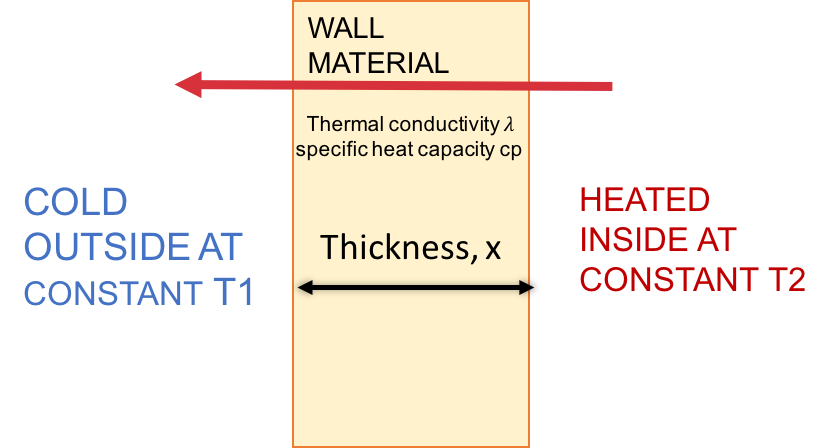
\includegraphics[width=8cm]{Fig_heat1/heat_cond_simple.png}
\end{figure}
Heat flow is important in the soil. To simplify, we're assuming heat flow through a wall. We test different insulation materials by assigning different heat capacities and thermal conductivity values of several real-world materials. 

In this tutorial three configuration files will be modified step by step. All configuration files are located in the folder \emph{drutes.conf} and respective subfolders. \begin{enumerate}
\item For selection of the module, dimension and time information we require \emph{global.conf}.  \emph{global.conf} is located in \emph{drutes.conf / global.conf}. 
\item To define the mesh or spatial discretization in 1D,  we require \emph{drumesh1D.conf}. \emph{drumesh1D.conf} is located in \emph{drutes.conf / mesh / drumesh1D.conf}. 
\item To define heat conduction, we require \emph{heat.conf}. \emph{heat.conf} is located in \emph{drutes.conf / heat / heat.conf}. 
\end{enumerate}
$DRUtES$ works with configuration input file with the file extension .conf. Blank lines and lines starting with \# are ignored. The input mentioned in this tutorial therefore needs to be placed one line below the mentioned keyword, unless stated otherwise. 



\newpage
\subsection{Scenarios}

For all scenarios, we assume that the wall is between a heated room, which is maintaining a constant temperature of 20 $^{\circ}$C, and the outside world during winter, which for the sake of simplicity is at a constant temperature of 0 $^{\circ}$C.

\begin{table}[!h]\caption{\label{tab_heat}Material properties needed for scenarios.}
\adjustbox{max height=\dimexpr\textheight-5cm\relax,
           max width=\textwidth}{

\small\begin{tabular}{l c c c}
\hline
& specific heat capacity & density & thermal conductivity\\
& c$_p$ &  $\rho$ & $\lambda$ \\
Material & [J kg$^{-1}$ K$^{-1}$] & [kg m$^{-3}$] & [W m$^{-1}$ K$^{-1}$  ] \\
 \hline
Stone concrete & 750 & 1400 & 1.7 \\
Sand stone & 920 & 2800 & 1.7 \\
Cotton &  1340& 1550 &0.04 \\
\hline
\end{tabular}
}
\end{table}


\section*{Scenario 1}

Heat conduction through a 20 cm thick stone concrete wall. 

$global.conf$: Choose correct model, dimension, time discretization and observation times.
\begin{enumerate}
\item Open \textbf{\emph{global.conf}} in a text editor of your choice. 
\item Model type: Your first input is the module. Input is \textbf{heat}.
\item Initial mesh configuration \begin{enumerate}
\item The dimension of our problem is 1. Input: 1.
\item We use the internal mesh generator. Input: 1. 
\end{enumerate}
\item Error criterion (not needed here, leave at default value) \begin{enumerate} 
\item Maximum number of iteration of the Picard method: 20 
\item h tolerance: 1e-2.
\end{enumerate}
\item Time information 
\begin{enumerate} 
%\item integration method is 3 point formula. Input: 30. 
\item Time units are in hours: input h
\item Initial time: 1e-3.
\item End time: 24.
\item Minimum time step: 1e-6.
\item Maximum time step: 0.1.
\end{enumerate}
\item Observation time settings \begin{enumerate}
\item Observation time method: 2
\item Set file format of observation: pure. Output in 1D is always in raw data. Different options will not impact output in 1D.
\item Make sequence of observation time: n
\item Number of observation times: 11
\item Observation time values: 2, 4, 6, 8, 10, 12 ,14, 16, 18, 20, 22. Use a new line for each input. \textit{DRUtES} automatically generates output for the initial time and final time. DRUtES will generate 13 output files, e.g. \textit{heat\_temperature-x.dat}, where x is the number of the file and not the output time. The initial time is assigned an x value of 0. 
\end{enumerate}
\item Observation point settings \begin{enumerate}
\item Observation point coordinates: 0.0, 0.2. Use a new line for each input. \textit{DRUtES} will generate 2 output files, e.g. \textit{obspt\_heat-x.out}, where x is the ID of the observation point. 
\end{enumerate}
\item Ignore other settings for now. 
\item Save $global.conf$
\end{enumerate}


$drumesh1D.conf$: Mesh definition, i.e. number of materials and spatial discretization
\begin{enumerate}
\item Open \textbf{\emph{drumesh1D.conf}} in a text editor of your choice. 
\item Geometry information: 0.2 m - domain length
\item Amount of intervals: 1
\item
\adjustbox{max height=\dimexpr\textheight-5cm\relax,
           max width=\textwidth}{
\small\begin{tabular}{|c | c | c|}
\hline
density & bottom & top \\
 \hline
0.005 & 0 & 0.2 \\
\hline
\end{tabular}
}
\item number of materials: 1
\item \adjustbox{max height=\dimexpr\textheight-5cm\relax,
           max width=\textwidth}{
\small\begin{tabular}{|c | c | c|}
\hline
id & bottom & top \\
 \hline
1& 0 & 0.2 \\
\hline
\end{tabular}
}
\end{enumerate}

\emph{heat.conf}: Heat module after Sophocleous (1979). 


\begin{enumerate}
\item Open \emph{heat.conf} in a text editor of your choice. 

\item Couple with Richards equation: n
\item Number of materials or layers: 1 
\item Specific heat capacity of the wall material: \\750 J kg$^{-1}$ K$^{-1}$ x 1400 kg m$^{-3}$ = 1.05E6 J m$^{-3}$ K$^{-1}$ = $\frac{1.05E6~\mathrm{W~s~m^{-3}~K^{-1}}}{3600~\mathrm{s~h^{-1}}}$ \\= 291 W h m$^{-3}$ K$^{-1}$. 
\item Specific heat capacity of liquid: 0
\item Anisotropy: There is no anisotropy. The value is 0.
\item Heat conductivity of the wall material: 1.7 W m$^{-1}$ K$^{-1}$. 
\item There is NO heat convection of water: 0.
\item The initial temperature is 0$^{\circ}$C across the entire domain: 0.
\item There is no heat source: 0. 
\item We have 2 boundaries at both ends of the wall. We assume a constant temperature of 0 $^{\circ}$C outside. We assume the inside is heated and the temperature maintained at exactly 20$^{\circ}$C. We therefore know the temperature at the boundaries. We also know that these values do not change in time. They can be describes as time-constant Dirichlet boundary conditions. \\
\adjustbox{max height=\dimexpr\textheight-5cm\relax,
           max width=\textwidth}{
\small\begin{tabular}{|c | c | c| c|}
\hline
boundary id & boundary type & use bc.dat & value \\
 \hline
101& 1 & n & 20.0 \\
102& 1 & n & 0.0 \\
\hline
\end{tabular}
}

\item Save heat.conf.
\end{enumerate}

\section*{Run scenario 1}
Run the simulation in the terminal console.
\begin{enumerate}
\item Make sure you are in the right directory. 
\item To execute $DRUtES$: \\
\$ bin/drutes
\item After the simulation finishes, to generate png plots execute provided R script: \\
\$ Rscript drutes.conf/heat/heatplots.R concrete
\item The output of the simulation can be found in the folder out
\end{enumerate}

\section*{Tasks for scenario 1}

\begin{enumerate}
\item How long does it take for the temperature distribution to become linear between the two observation points?
\item How large is the steady state heat flux through the wall?
\item Let's assume a wall area of A=15 m$^2$. Use the observation point at the boundary between the wall and the inside of room. How large was the cumulated heat loss 24 h. How much will be lost after 48 h when the set-up does not change?
\end{enumerate}


\section*{Result of scenario 1}

\subsection*{Question 1}
Figure \ref{plot1} shows that the temperature distribution becomes linear quite quickly and reaches a steady state after observation time 2, which was set to 4 h. Figure \ref{plot2} shows the heat flux $\phi_{\mathrm{p}}$ in observation points 1 (red) and 2 (blue) bordering the wall to the outside and heated inside, respectively.  The heat flux is extremely large at observation point 2 in the beginning. Observation point 2 evidently defines the boundary between the wall and the heated inside. After approximately 3 hours, the heat flux of observation point 1 and 2 become identical. This occurs when the simulation reaches steady state and a linear temperature distribution. Figure \ref{plot2} allows a more exact estimation of when the system becomes steady state. 

\begin{figure}[!h]
\centering
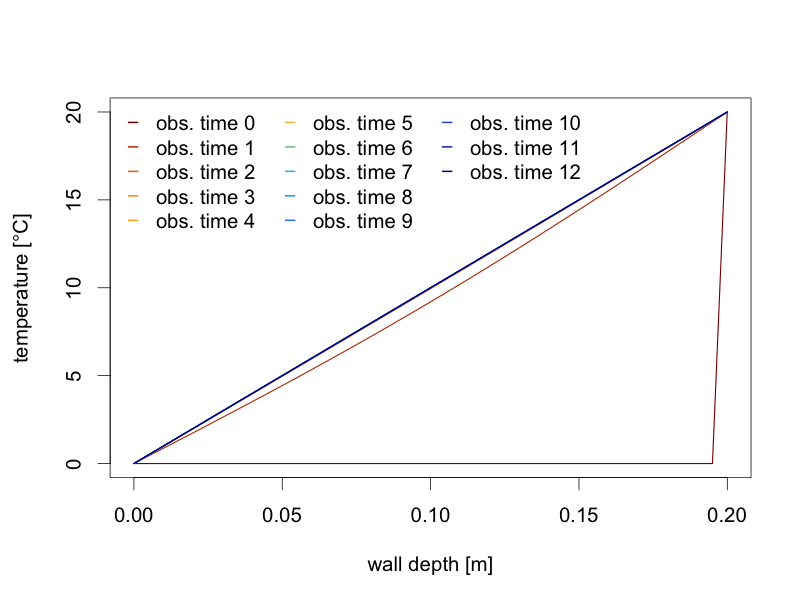
\includegraphics[width=10.5cm]{Fig_heat1/obs_time_temp_concrete.png}
\caption{\label{plot1}Plot of observation times for stone concrete generated with Rscript heatplots.R}
\end{figure}

\subsection*{Question 2}

\begin{figure}[!h]
\centering
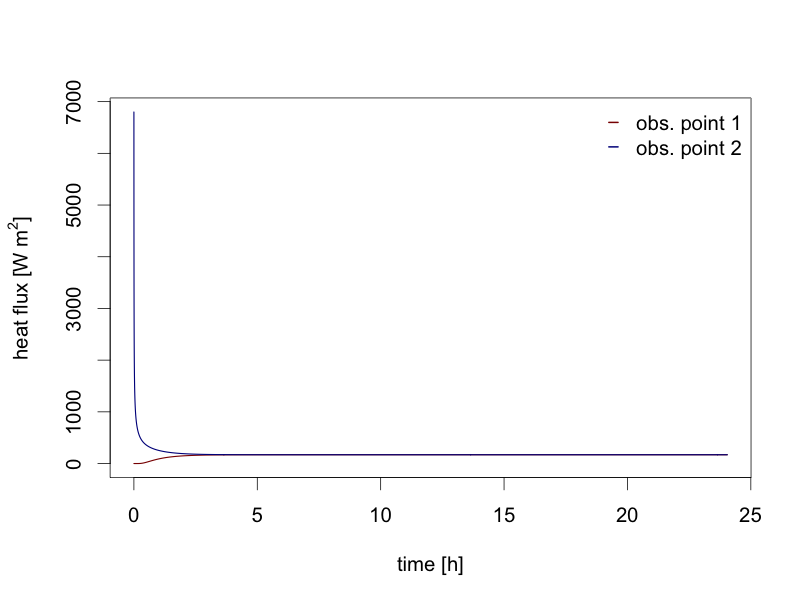
\includegraphics[width=10.5cm]{Fig_heat1/obs_point_temp_concrete.png}
\caption{\label{plot2} Heat flux at observation points 1 and 2 for stone concrete generated with Rscript heatplots.R}
\end{figure}

The constant heat flux value is at $\phi_{p}$=170 W m$^{-2}$. This value can also be calculated using the equation:
\begin{equation*}
\phi_{\mathrm{p}}=-\lambda\frac{dT}{dx}= -1.7 \frac{20-0}{0.2}= 170 \mathrm{~W~m^{-2}}
\end{equation*}

\newpage
\subsection*{Question 3}

Figure \ref{plot3} shows the cumulative heat flux in observation points 1 and 2, both ends of the wall. The cumulative heat flux after 24 h at observation point is 4468 W m$^{-2}$. With a wall area of 15 m$^2$ this results in $Q = 4468~\mathrm{W~h~m^{-2}}\cdot~15~\mathrm{m^{2}}= 67020 ~\mathrm{W~h}$. 
For the next 24 h, the heat flux will be constant at 170 $\mathrm{~W~m^{-2}}$. The total heat loss will therefore be $Q=170 \mathrm{~W~m^{-2}}~\cdot 24~\mathrm{h}~\cdot~15~\mathrm{m^{2}}=61200 \mathrm{~W~h}$.

\begin{figure}[!h]
\centering
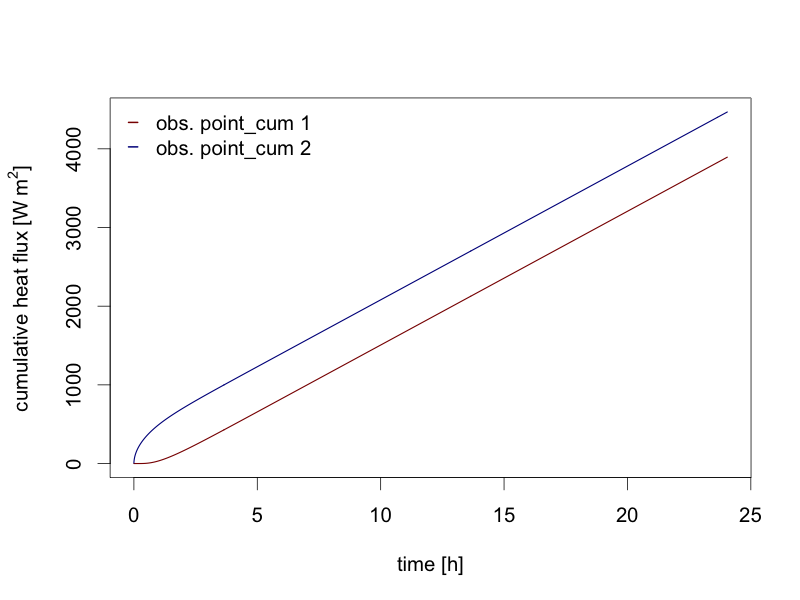
\includegraphics[width=10.5cm]{Fig_heat1/obs_point_cum_temp_concrete.png}
\caption{\label{plot3} Cumulated heat flux at observation points 1 and 2 for stone concrete generated with Rscript heatplots.R}
\end{figure}

\newpage

\section*{Scenario 2}
Heat conduction through a 20 cm thick sandstone wall. 

\begin{enumerate}
\item Open \emph{heat.conf} in a text editor of your choice. 
\item Leave all settings the same, except for specific heat capacity. 
\item Replace the specific heat capacity with values of sand stone.
\item Save heat.conf.
\end{enumerate}

\section*{Run scenario 2}
Run the simulation in the terminal console.
\begin{enumerate}
\item Make sure you are in the right directory. 
\item To execute $DRUtES$: \\
\$ bin/drutes
\item After the simulation finishes, to generate png plots execute provided R script: \\
\$ Rscript drutes.conf/heat/heatplots.R sandstone
\item The output of the simulation can be found in the folder out
\end{enumerate}

\section*{Tasks for scenario 2}

\begin{enumerate}
\item Answer the same questions as for scenario 1. What is different?
\end{enumerate}

\section*{Result of scenario 2}
\subsection*{Question 1}
Figure \ref{plot4} shows that it takes longer for the temperature distribution to become linear in sandstone than in concrete sand. Also taking Fig. \ref{plot5} into account, it takes approximately 5 h. This is because sandstone has a larger specific heat capacity than stone concrete.

\begin{figure}[!h]
\centering
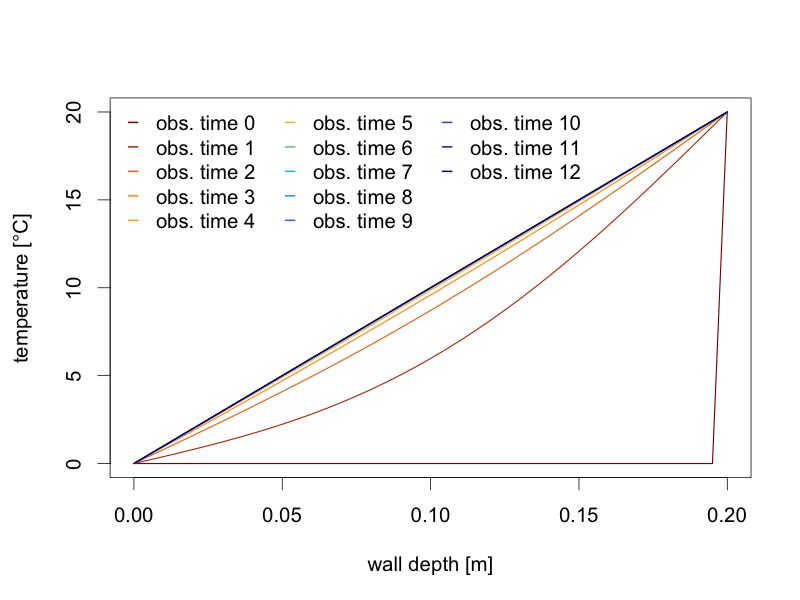
\includegraphics[width=10.5cm]{Fig_heat1/obs_time_temp_sandstone.png}
\caption{\label{plot4}Plot of observation times for sandstone generated with Rscript heatplots.R}
\end{figure}

\subsection*{Question 2}

The constant heat flux when the system is in steady state is also at $\phi_{p}$=170 W m$^{-2}$. Both materials have the same thermal conductivity and therefore the same thermal heat flux.

\begin{figure}[!h]
\centering
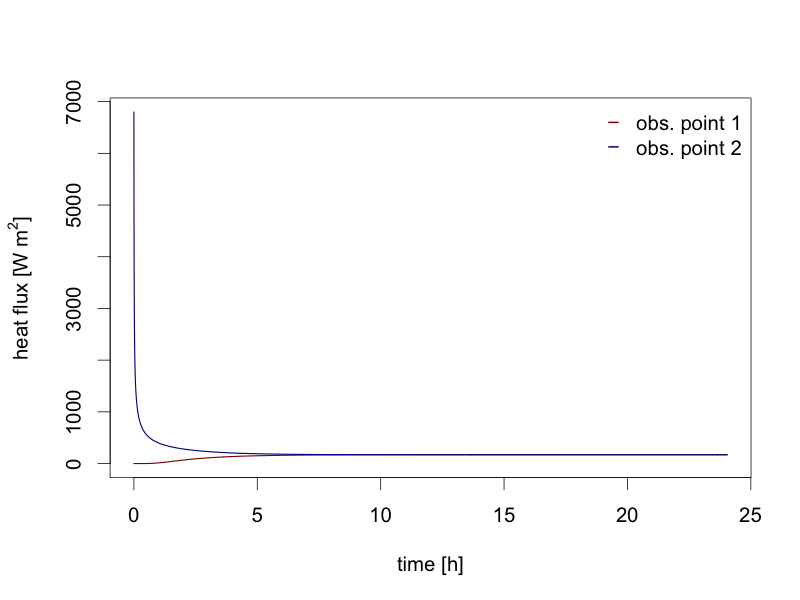
\includegraphics[width=10.5cm]{Fig_heat1/obs_point_temp_sandstone.png}
\caption{\label{plot5} Heat flux at observation points 1 and 2 for sandstone generated with Rscript heatplots.R}
\end{figure}


\subsection*{Question 3}
Heat conduction through a 20 cm thick cotton fibre wall. 

The cumulative heat flux after 24 h at observation point 2 in sandstone is higher than in concrete stone, namely 5014 W m$^{-2}$. With a wall area of 15 m$^2$ this results in $Q = 5014~\mathrm{W~h~m^{-2}}\cdot~15~\mathrm{m^{2}}= 75210 ~\mathrm{W~h}$. 
For the next 24 h, the heat flux will be constant at 170 $\mathrm{~W~m^{-2}}$. The total heat loss will therefore also be $Q=170 \mathrm{~W~m^{-2}}~\cdot 24~\mathrm{h}~\cdot~15~\mathrm{m^{2}}=61200 \mathrm{~W~h}$.

\begin{figure}[!h]
\centering
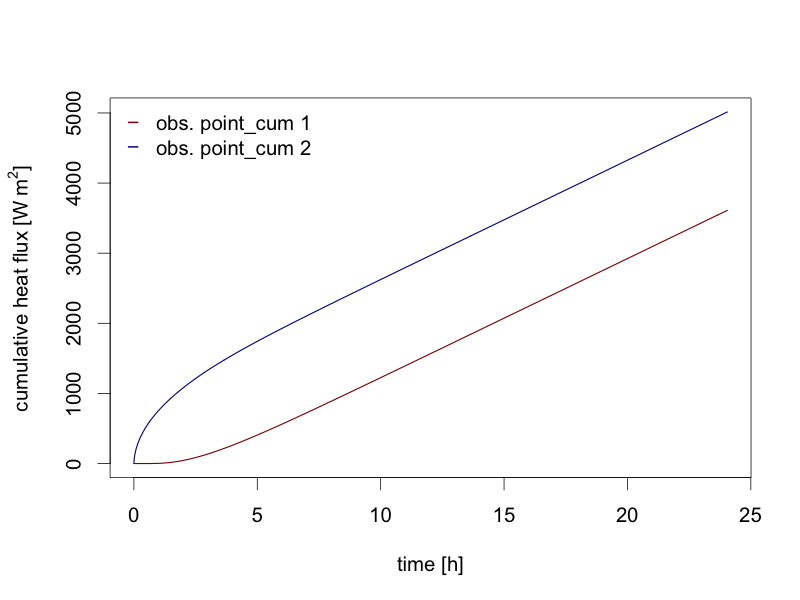
\includegraphics[width=10.5cm]{Fig_heat1/obs_point_cum_temp_sandstone.png}
\caption{\label{plot6} Cumulated heat flux at observation points 1 and 2 for sandstone generated with Rscript heatplots.R}
\end{figure}

\newpage
\newpage
\newpage
\clearpage
\section*{Scenario 3}

\begin{enumerate}
\item Open \emph{heat.conf} in a text editor of your choice. 
\item Change the specific heat capacity and thermal conductivity with values of cotton.
\item Save heat.conf.
\end{enumerate}

\section*{Run scenario 3}
Run the simulation in the terminal console.
\begin{enumerate}
\item Make sure you are in the right directory. 
\item To execute $DRUtES$: \\
\$ bin/drutes
\item After the simulation finishes, to generate png plots execute provided R script: \\
\$ Rscript drutes.conf/heat/heatplots.R cotton
\item The output of the simulation can be found in the folder out
\end{enumerate}

\section*{Tasks for scenario 3}

\begin{enumerate}
\item Answer the same questions as for scenario 1. What is different to scenario 1 and 2?
\end{enumerate}

\section*{Result of scenario 3}
\subsection*{Question 1}
In contrary to scenario 1 and 2, figure \ref{plot7} and \ref{plot8} show that we have not reached steady-state within 24 h. This is because of the very low thermal heat conductivity of cotton fibre. 

\begin{figure}[!h]
\centering
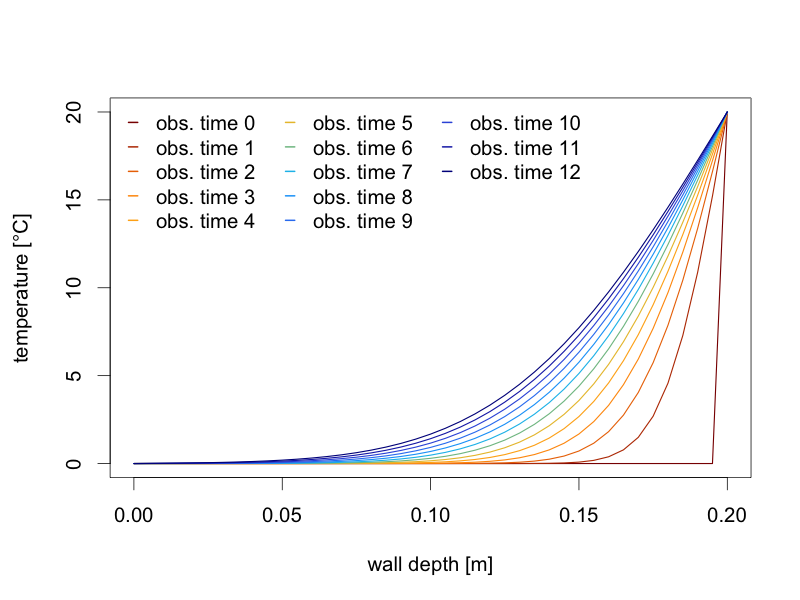
\includegraphics[width=10.5cm]{Fig_heat1/obs_time_temp_cotton.png}
\caption{\label{plot7}Plot of observation times for cotton generated with Rscript heatplots.R}
\end{figure}

\subsection*{Question 2}

\begin{figure}[!h]
\centering
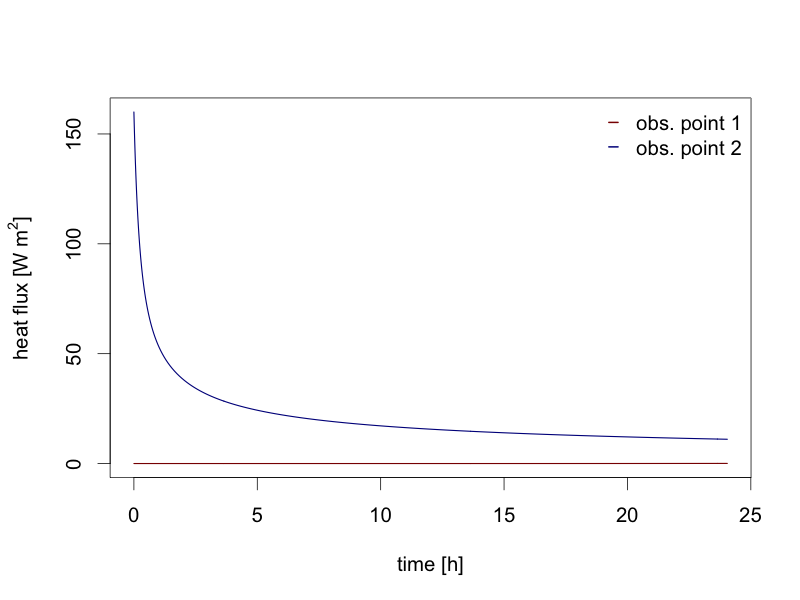
\includegraphics[width=10.5cm]{Fig_heat1/obs_point_temp_cotton.png}
\caption{\label{plot8} Heat flux at observation points 1 and 2 for cotton generated with Rscript heatplots.R}
\end{figure}

We cannot estimate the constant heat flux during steady-state with our results. Using the heat flux equation mentioned during scenario 1, we can calculate the heat flux during steady state:
\begin{equation*}
\phi_{\mathrm{p}}=-\lambda\frac{dT}{dx}= -0.04 \frac{20-0}{0.2}= 4 \mathrm{~W~m^{-2}}
\end{equation*}

\subsection*{Question 3}

The cumulative heat flux after 24 h at observation point 2 in sandstone is higher than in concrete stone, namely 503 W m$^{-2}$, so about a tenth of sandstone and stone concrete. With a wall area of 15 m$^2$ this results in $Q = 503~\mathrm{W~h~m^{-2}}\cdot~15~\mathrm{m^{2}}= 7545 ~\mathrm{W~h}$. 

Since the system is not in steady state, it is difficult to estimate the heat loss for the next 24 h. The answer has to be evaluated numerically by increasing the end time to 48 h. 

\begin{figure}[!h]
\centering
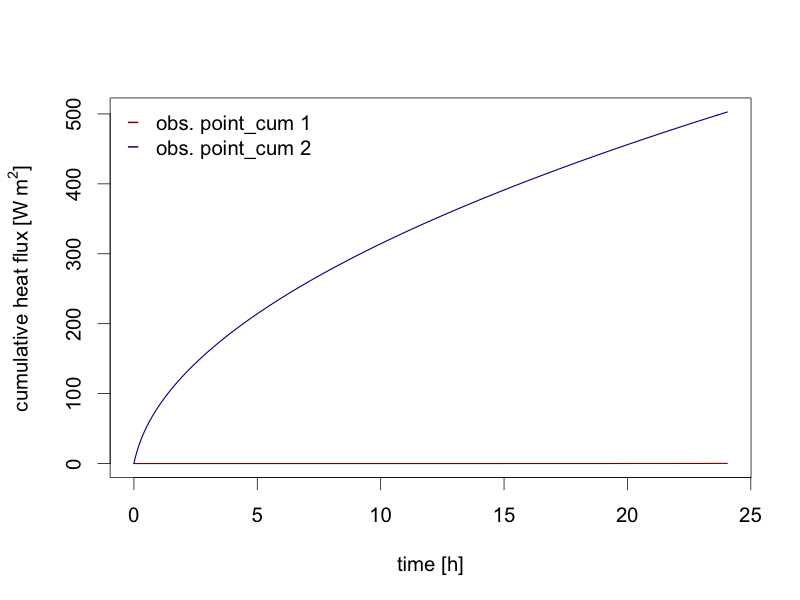
\includegraphics[width=10.5cm]{Fig_heat1/obs_point_cum_temp_cotton.png}
\caption{\label{plot9} Cumulated heat flux at observation points 1 and 2 for sandstone generated with Rscript heatplots.R}
\end{figure}

\newpage
\newpage

\subsection{Outcome}
\begin{enumerate}
\item You got familiar with the $DRUtES$ heat module in 1D.
\item You simulated heat conduction through a wall with different materials
\item You understand the effects of different heat capacities and thermal conductivities.
\item You understand the term \emph{Dirichlet boundary condition}, \emph{initial condition} and \emph{steady state}.
\end{enumerate}

\section{Heat module - Part 2}
\subsection{Goal and Complexity}
\subsection*{Complexity: Beginner}

\subsection*{Prerequisites: Tutorial: heat module - part 1.}

The goal of this tutorial is to show further applicability of the $DRUtES$ heat module in 1D. We simulate heat conduction in a wall with two materials to understand the effects of layering of materials with different thermal properties.\medskip

\begin{figure}[!h]
\centering
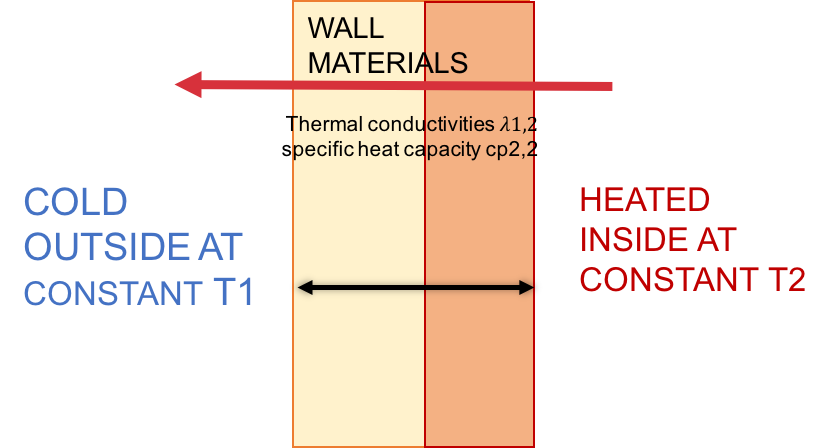
\includegraphics[width=8cm]{Fig_heat2/heat_cond_simple.png}
\end{figure}

Similar to tutorial 1, three configuration files will be modified step by step. All configuration files are located in the folder \emph{drutes.conf} and respective subfolders. \begin{enumerate}
\item For selection of the module, dimension and time information we require \emph{global.conf}.  \emph{global.conf} is located in \emph{drutes.conf / global.conf}. 
\item To define the mesh or spatial discretization in 1D,  we require \emph{drumesh1D.conf}. \emph{drumesh1D.conf} is located in \emph{drutes.conf / mesh / drumesh1D.conf}. 
\item To define heat conduction, we require \emph{heat.conf}. \emph{heat.conf} is located in \emph{drutes.conf / heat / heat.conf}. 
\end{enumerate}
$DRUtES$ works with configuration input file with the file extension .conf. Blank lines and lines starting with \# are ignored. The input mentioned in this tutorial therefore needs to be placed one line below the mentioned keyword, unless stated otherwise. 

\newpage
\subsection{Scenarios}

For all scenarios, we assume that the wall is between a heated room, which is maintaining a constant temperature of 20 $^{\circ}$C, and the outside world during winter, which for the sake of simplicity is at a constant temperature of 0 $^{\circ}$C.

\begin{table}[!h]\caption{\label{tab_heat2}Material properties needed for scenarios.}
\adjustbox{max height=\dimexpr\textheight-5cm\relax,
           max width=\textwidth}{

\small\begin{tabular}{l c c c}
\hline
& specific heat capacity & density & thermal conductivity\\
& c$_p$ &  $\rho$ & $\lambda$ \\
Material & [J kg$^{-1}$ K$^{-1}$] & [kg m$^{-3}$] & [W m$^{-1}$ K$^{-1}$  ] \\
 \hline
Stone concrete & 750 & 1400 & 1.7 \\
Cotton &  1340& 1550 &0.04 \\
\hline
\end{tabular}
}
\end{table}


\section*{Scenario 1}

Heat conduction through a 20 cm wall. 15 cm are made of stone concrete and 5 cm are made of cotton fibre.

$global.conf$: Choose correct model, dimension, time discretization and observation times. This is the same as in heat tutorial 1.
\begin{enumerate}
\item Open \textbf{\emph{global.conf}} in a text editor of your choice. 
\item Model type: Your first input is the module. Input is \textbf{heat}.
\item Initial mesh configuration \begin{enumerate}
\item The dimension of our problem is 1. Input: 1.
\item We use the internal mesh generator. Input: 1. 
\end{enumerate}
\item Error criterion (not needed here, leave at default value) \begin{enumerate} 
\item Maximum number of iteration of the Picard method: 20 
\item h tolerance: 1e-2.
\end{enumerate}
\item Time information 
\begin{enumerate} 
%\item integration method is 3 point formula. Input: 30. 
\item Time units are in hours: input h
\item Initial time: 1e-3.
\item End time: 24.
\item Minimum time step: 1e-6.
\item Maximum time step: 0.1.
\end{enumerate}
\item Observation time settings \begin{enumerate}
\item Observation time method: 2
\item Set file format of observation: pure. Output in 1D is always in raw data. Different options will not impact output in 1D.
\item Make sequence of observation time: n
\item Number of observation times: 11
\item Observation time values: 2, 4, 6, 8, 10, 12 ,14 ,16, 18, 20, 22. Use a new line for each input. \textit{DRUtES} automatically generates output for the initial time and final time. DRUtES will generate 13 output files, e.g. \textit{heat\_temperature-x.dat}, where x is the number of the file and not the output time. The initial time is assigned an x value of 0. 
\end{enumerate}
\item Observation point settings \begin{enumerate}
\item Observation point coordinates: 0.0, 0.2. Use a new line for each input. \textit{DRUtES} will generate 2 output files, e.g. \textit{obspt\_heat-x.out}, where x is the ID of the observation point. 
\end{enumerate}
\item Ignore other settings for now. 
\item Save $global.conf$
\end{enumerate}


$drumesh1D.conf$: Mesh definition, i.e. number of materials and spatial discretization. Here is were the configuration files are different to heat tutorial one. 
\begin{enumerate}
\item Open \textbf{\emph{drumesh1D.conf}} in a text editor of your choice. 
\item Geometry information: 0.2 m - domain length
\item Amount of intervals: 1
\item
\adjustbox{max height=\dimexpr\textheight-5cm\relax,
           max width=\textwidth}{
\small\begin{tabular}{|c | c | c|}
\hline
density & bottom & top \\
 \hline
0.005 & 0 & 0.2 \\
\hline
\end{tabular}
}
\item Number of materials: 2
\item \adjustbox{max height=\dimexpr\textheight-5cm\relax,
           max width=\textwidth}{
\small\begin{tabular}{|c | c | c|}
\hline
id & bottom & top \\
 \hline
1& 0 & 0.15 \\
2 & 0.15 &0.2 \\
\hline
\end{tabular}
}
\end{enumerate}

\emph{heat.conf}: Heat module after Sophocleous (1979). 
Here, it is important to make sure everything is defined for 2 layers. 2 lines of input are required, even when the input is identical. 

\begin{enumerate}
\item Open \emph{heat.conf} in a text editor of your choice. 
\item Couple with Richards equation: n
\item Number of materials or layers: 2
\item Specific heat capacity of the wall material: 
Material 1 is stone concrete: \\750 J kg$^{-1}$ K$^{-1}$ x 1400 kg m$^{-3}$ = 1.05E6 J m$^{-3}$ K$^{-1}$ = $\frac{1.05E6~\mathrm{W~s~m^{-3}~K^{-1}}}{3600~\mathrm{s~h^{-1}}}$ \\= 291 W h m$^{-3}$ K$^{-1}$. \\
Material 2 is cotton fibre: \\1340 J kg$^{-1}$ K$^{-1}$ x 1550 kg m$^{-3}$ = 2.08E6 J m$^{-3}$ K$^{-1}$ = $\frac{2.08E6~\mathrm{W~s~m^{-3}~K^{-1}}}{3600~\mathrm{s~h^{-1}}}$ \\= 576 W h m$^{-3}$ K$^{-1}$. 
\item Specific heat capacity of liquid: 0 (for both materials)
\item Anisotropy: There is no anisotropy. The value is 0 (for both materials)
\item Heat conductivity of the wall material: \\ Material 1: 1.7 W m$^{-1}$ K$^{-1}$ \\ Material 2: 0.04 W m$^{-1}$ K$^{-1}$
\item There is NO heat convection of water: 0 (for both materials)
\item The initial temperature is 0$^{\circ}$C across the entire domain: 0 (for both materials)
\item There is no heat source: 0 (for both materials)
\item This is identical to heat tutorial 1. We have 2 boundaries at both ends of the wall. We assume a constant temperature of 0$^{\circ}$C outside. We assume the inside is heated and the temperature maintained at exactly 20$^{\circ}$C. We therefore know the temperature at the boundaries. We also know that these values do not change in time. They can be describes as time-constant Dirichlet boundary conditions. \\
\adjustbox{max height=\dimexpr\textheight-5cm\relax,
           max width=\textwidth}{
\small\begin{tabular}{|c | c | c| c|}
\hline
boundary id & boundary type & use bc.dat & value \\
 \hline
101& 1 & n & 20.0 \\
102& 1 & n & 0.0 \\
\hline
\end{tabular}
}

\item Save heat.conf.
\end{enumerate}

\section*{Run scenario 1}
Run the simulation in the terminal console.
\begin{enumerate}
\item Make sure you are in the right directory. 
\item To execute $DRUtES$: \\
\$ bin/drutes
\item After the simulation finishes, to generate png plots execute provided R script: \\
\$ Rscript drutes.conf/heat/heatplots.R concretecotton1
\item The output of the simulation can be found in the folder out

\end{enumerate}

\section*{Tasks for scenario 1}

\begin{enumerate}
\item Describe the temperature distribution. How long does it take for the temperature distribution to become linear between the two observation points?
\item How large is the steady state heat flux through the wall?
\item Let's assume a wall area of A=15 m$^2$. Use the observation point at the boundary between the wall and the inside of room. How large was the cumulated heat loss 24 h. How much will be lost after 48 h when the set-up does not change?
\end{enumerate}


\section*{Result of scenario 1}

\subsection*{Question 1}
Figure \ref{plot1h} shows two distinct linear temperature distributions. The temperature distributions appears to have not changed significantly over the last observation times indicating a steady state. A 5 cm thick cotton fibre wall is between the concrete stone and the heated inside. The overall heat flux at the inside border is therefore quite low as the input of heat has to travel through badly conducting material first. 

\begin{figure}[!h]
\centering
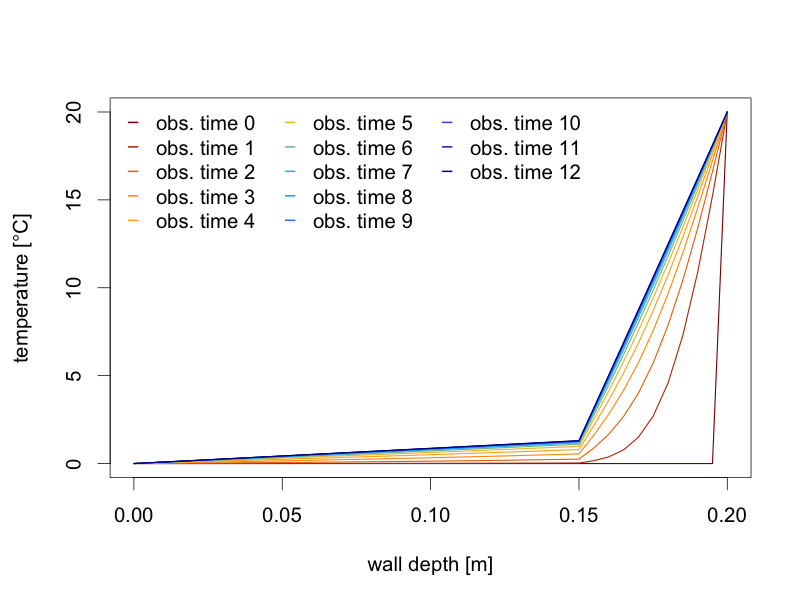
\includegraphics[width=10.5cm]{Fig_heat2/obs_time_temp_concretecotton1.png}
\caption{\label{plot1h}Plot of observation times for a wall with a 15 cm outer stone concrete layer and an inner 5 cm cotton fibre layer  generated with Rscript heatplots.R}
\end{figure}

\subsection*{Question 2}

\begin{figure}[!h]
\centering
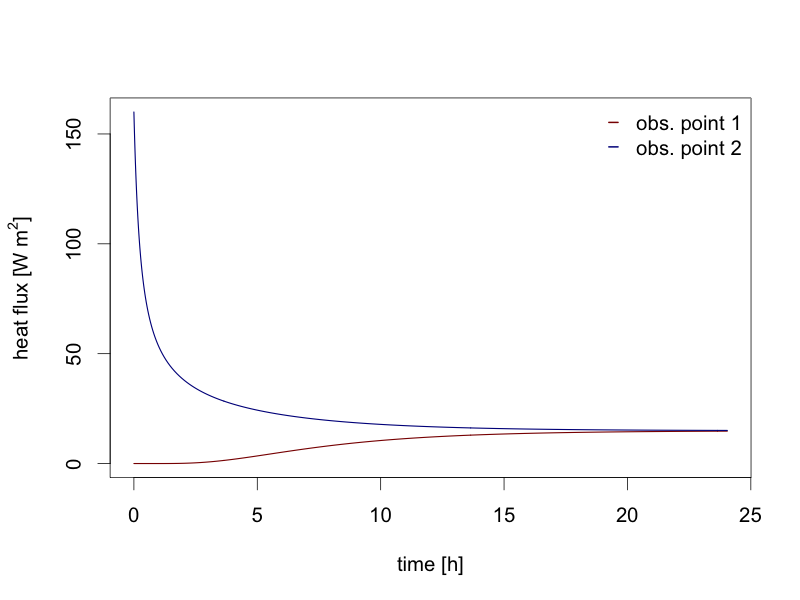
\includegraphics[width=10.5cm]{Fig_heat2/obs_point_temp_concretecotton1.png}
\caption{\label{plot2h} Heat flux at observation points 1 and 2 for a wall with a 15 cm outer stone concrete layer and an inner 5 cm cotton fibre layer generated with Rscript heatplots.R}
\end{figure}

Looking at the raw data, it appears that steady-state has not actually been reached, but that the change in heat flux is becoming slower and is converging towards 15 W m$^{-2}$. 

\newpage
\subsection*{Question 3}

Figure \ref{plot3h} shows the cumulative heat flux in observation points 1 and 2, both ends of the wall. The cumulative heat flux after 24 h at observation point is 538 W m$^{-2}$. With a wall area of 15 m$^2$ this results in $Q = 538~\mathrm{W~h~m^{-2}}\cdot~15~\mathrm{m^{2}}= 8070 ~\mathrm{W~h}$. 
For the next 24 h, the heat flux will be constant at 15 $\mathrm{~W~m^{-2}}$. The total heat loss will therefore be $Q=15 \mathrm{~W~m^{-2}}~\cdot 24~\mathrm{h}~\cdot~15~\mathrm{m^{2}}=5400 \mathrm{~W~h}$.

\begin{figure}[!h]
\centering
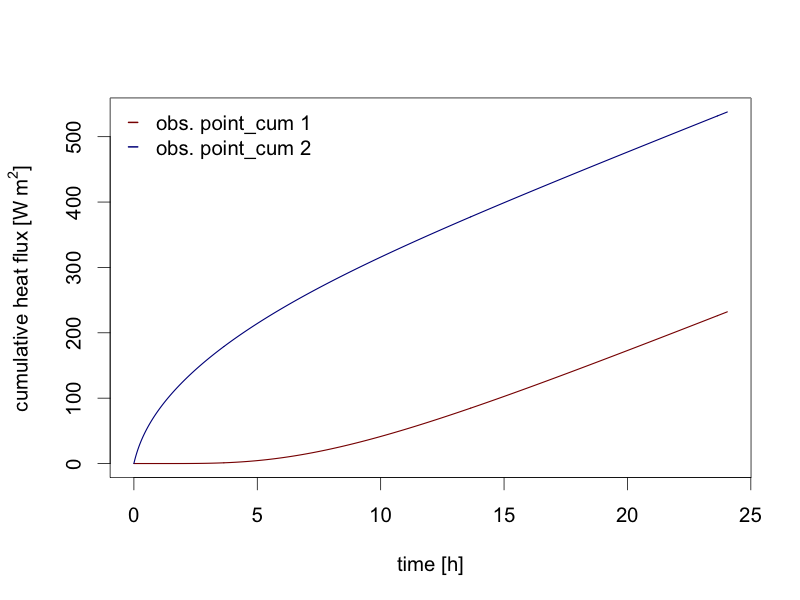
\includegraphics[width=10.5cm]{Fig_heat2/obs_point_cum_temp_concretecotton1.png}
\caption{\label{plot3h} Cumulated heat flux at observation points 1 and 2 for a wall with a 15 cm outer stone concrete layer and an inner 5 cm cotton fibre layer generated with Rscript heatplots.R}
\end{figure}

\newpage

\section*{Scenario 2}

\begin{enumerate}
\item Open \emph{heat.conf} in a text editor of your choice. 
\item Swap the order of materials for specific heat capacity and thermal conductivity. Now, the the outer wall layer is made of cotton fibre and the inner layer is made of concrete.
\item Save heat.conf.
\end{enumerate}

\section*{Run scenario 2}
Run the simulation in the terminal console.
\begin{enumerate}
\item Make sure you are in the right directory. 
\item To execute $DRUtES$: \\
\$ bin/drutes
\item After the simulation finishes, to generate png plots execute provided R script: \\
\$ Rscript drutes.conf/heat/heatplots.R cottonconcrete
\item The output of the simulation can be found in the folder out

\end{enumerate}

\section*{Tasks for scenario 2}

\begin{enumerate}
\item Answer the same questions as for scenario 1. What is different?
\end{enumerate}

\section*{Result of scenario 2}
\subsection*{Question 1}
Figure \ref{plot4h} shows the inner concrete layer becomes linear quite quickly, but that the outer cotton fibre layer has not reached linearity after 24 h. Also taking Fig. \ref{plot5h2} 
\begin{figure}[!h]
\centering
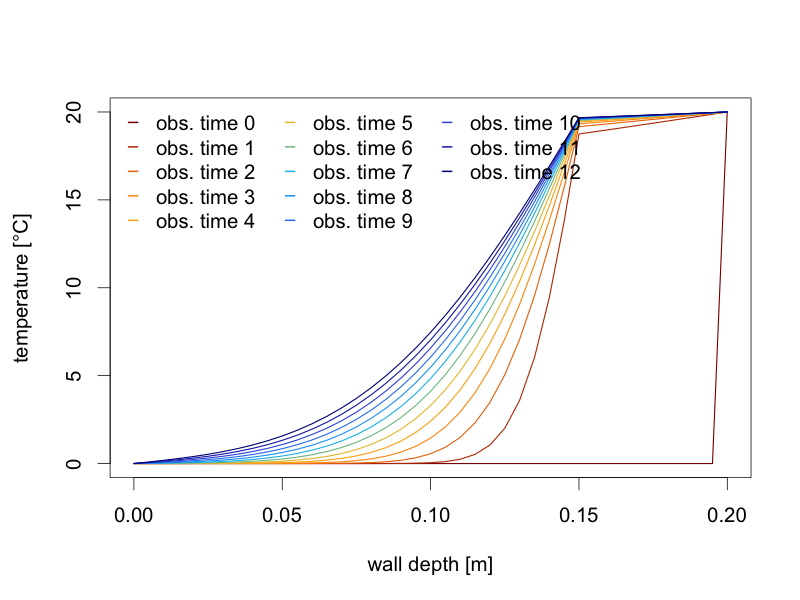
\includegraphics[width=10.5cm]{Fig_heat2/obs_time_temp_concretecotton2.png}
\caption{\label{plot4h}Plot of observation times for a wall with a 15 cm thick outer cotton layer and a 5 cm inner concrete stone layer generated with Rscript heatplots.R}
\end{figure}

\subsection*{Question 2}

The system has not reached a constant heat flux, but the heat flux will be between 0.7 and 111 W m$^{-2}$. A long simulation (not shown) of 240 h shows that the steady state hea flux converges towards 53 W m$^{-2}$.

\begin{figure}[!h]
\centering
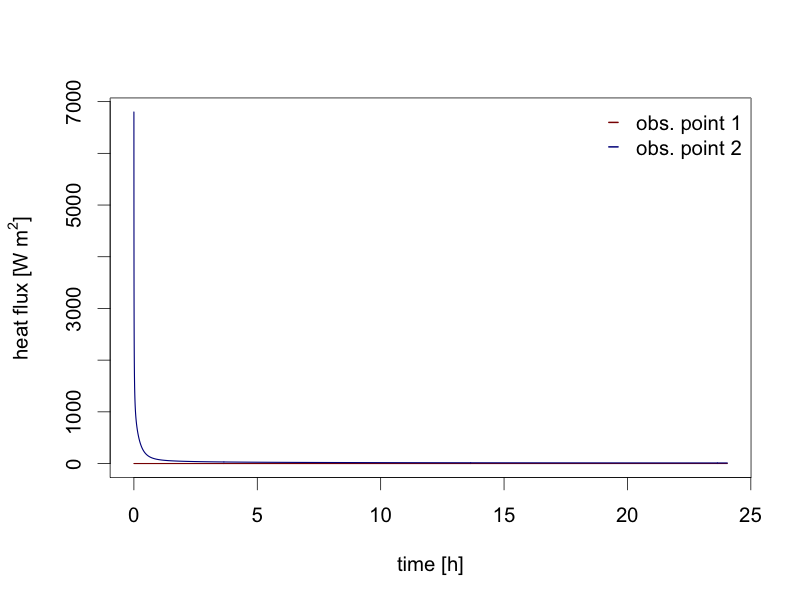
\includegraphics[width=10.5cm]{Fig_heat2/obs_point_temp_concretecotton2.png}
\caption{\label{plot5h2} Heat flux at observation points for a wall with a 15 cm thick outer cotton layer and a 5 cm inner concrete stone layer generated with Rscript heatplots.R}
\end{figure}


\subsection*{Question 3}

The cumulative heat flux after 24 h at the inner boundary is higher than in scenario 1, namely 797 W m$^{-2}$. With a wall area of 15 m$^2$ this results in $Q = 797~\mathrm{W~h~m^{-2}}\cdot~15~\mathrm{m^{2}}= 11955 ~\mathrm{W~h}$. 
For the next 24 h, the heat flux will not be constant and needs to be numerically simulated. 

\begin{figure}[!h]
\centering
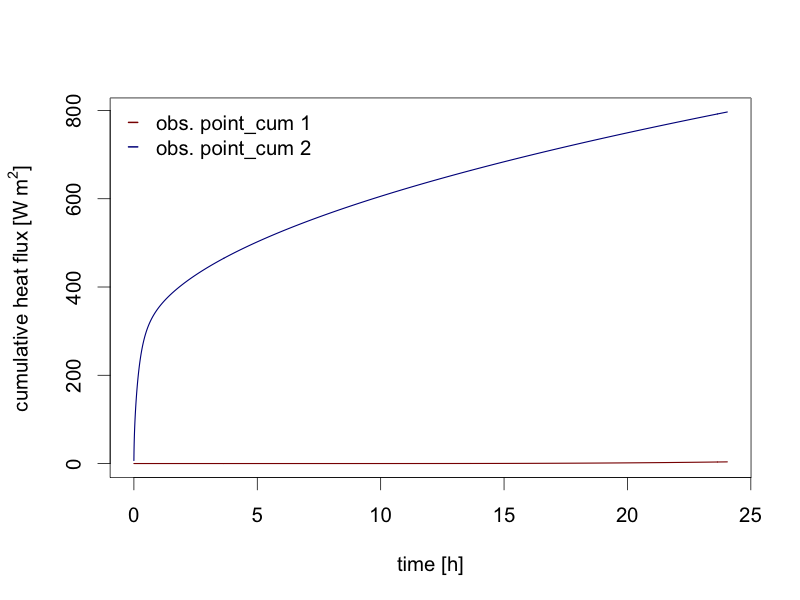
\includegraphics[width=10.5cm]{Fig_heat2/obs_point_cum_temp_concretecotton2.png}
\caption{\label{plot6h2} Cumulated heat flux at observation points for a wall with a 15 cm thick outer cotton layer and a 5 cm inner concrete stone layer generated with Rscript heatplots.R}
\end{figure}

\newpage
\newpage
\newpage

\subsection{Outcome}
\begin{enumerate}
\item You got familiar with the $DRUtES$ heat module in 1D with 2 layers.
\item You simulated heat conduction through a wall with layered materials.
\item You understand the effects of layering of materials with different heat capacities and thermal conductivities.
\item You understand how layering affects when a system is in \emph{steady state}.
\end{enumerate}
--
\resetlinenumber
\chapter{Water flow module}

\section{Infiltration - Part 1}
\subsection{Goal and Complexity}
\subsubsection*{Complexity: Beginner}

\subsubsection*{Prerequisites: None}

The goal of this tutorial is to get familiar with the $DRUtES$ standard Richards equation module and $DRUtES$ configuration in 1D by simulating infiltration into different soil \medskip

\begin{figure}[!h]
\centering
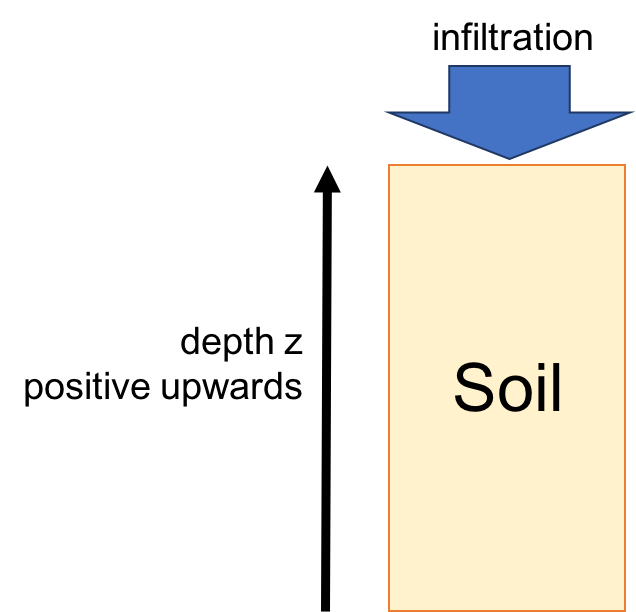
\includegraphics[width=8cm]{Fig_inf1/infilt.png}
\end{figure}
The process of infiltration is fundamental and yet very important in soil science. Infiltration into the soil determines water, heat and contaminant transport. Infiltration experiments can be used to determine some parameters describing soil hydraulic properties. 

In this tutorial three configuration files will be modified step by step. All configuration files are located in the folder \emph{drutes.conf} and respective subfolders. \begin{enumerate}
\item For selection of the module, dimension and time information we require \emph{global.conf}.  \emph{global.conf} is located in \emph{drutes.conf / global.conf}. 
\item To define the mesh or spatial discretization in 1D,  we require \emph{drumesh1D.conf}. \emph{drumesh1D.conf} is located in \emph{drutes.conf / mesh / drumesh1D.conf}. 
\item To define the infiltration, we require \emph{matrix.conf}. \emph{matrix.conf} is located in \emph{drutes.conf /water.conf/ matrix.conf}. 
\end{enumerate}
$DRUtES$ works with configuration input file with the file extension .conf. Blank lines and lines starting with \# are ignored. The input mentioned in this tutorial therefore needs to be placed one line below the mentioned keyword, unless stated otherwise. 

\newpage
\subsection{Scenarios}

We are using the well-known van Genuchten-Mualem parameterization to describe the soil hydraulic properties of our soils. The parameters describe clay, silt and sand (Tab. \ref{tab_inf1}). We assume a constant flow of water infiltrating over the top boundary. We can also look at this as a constant rate of water and it therefore describes the temporal derivative. This type of boundary is called a \textbf{Neumann condition}. We assume that the groundwater table is at the bottom of our profile. We therefore assume a constant state of saturation at the bottom profile. In these scenarios we want to investigate the effect of spatial and temporal discretization.

\begin{table}[!h]
\centering
\caption{\label{tab_inf1}Material properties needed for scenarios.}
\adjustbox{max height=\dimexpr\textheight-2cm\relax,
           max width=\textwidth}{

\small\begin{tabular}{l l c c c c c c}
\hline
Parameter & Description & Sand & Silt & Clay\\
\hline

$\alpha$ [cm$^{-1}$]& inverse of the air entry value &0.10 &0.08&0.01 \\
 $n$ [-]& shape parameter &2.2  & 1.8&1.5  \\
 $m$ [-]& shape parameter &0.55  & 0.44 & 0.33  \\
  $ \theta_s$ [-]&saturated vol. water content&0.4  & 0.45 & 0.5  \\
  $ \theta_r$ [-]& residual vol. water content&0.0 & 0.05 & 0.1  \\
  $Ss$ [cm$^{-1}$] & specific storage & 1e-9 & 1e-9 & 1e-10 \\
  $K_s$ [cm d$^{-1}$] & saturated hydraulic conductivity & 400 & 40 & 4 \\ 
\hline
\end{tabular}
}
\end{table}
\begin{figure}[!h]
\centering
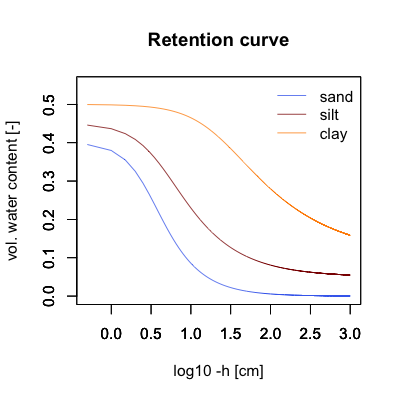
\includegraphics[width=6cm]{Fig_inf1/retention_curve.png}
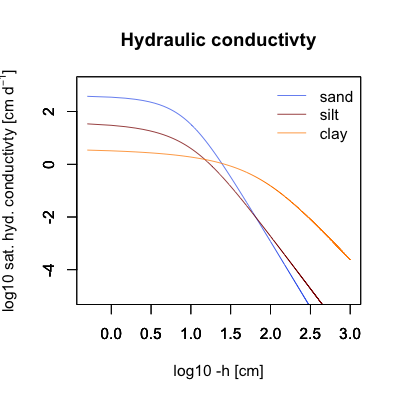
\includegraphics[width=6cm]{Fig_inf1/cond_hyd_curve.png}
\end{figure}

\section*{Scenario 1}

Infiltration into sandy soil. 

$global.conf$: Choose correct model, dimension, time discretization and observation times.
\begin{enumerate}
\item Open \textbf{\emph{global.conf}} in a text editor of your choice. 
\item Model type: Your first input is the module. Input is \textbf{RE}.
\item Initial mesh configuration \begin{enumerate}
\item The dimension of our problem is 1. Input: 1.
\item We use the internal mesh generator. Input: 1.
\end{enumerate}
\item Error criterion \begin{enumerate} 
\item Maximum number of iteration of the Picard method: 20.
\item h tolerance: 1e-1.
\end{enumerate}
\item Time information 
\begin{enumerate} 
%\item integration method is 3 point formula. Input: 30. 
\item Time units are in hours: input d.
\item Initial time: 1e-4.
\item End time: 1.
\item Minimum time step: 1e-4.
\item Maximum time step: 0.1.
\end{enumerate}
\item Observation time settings \begin{enumerate}
\item Observation time method: 2.
\item Set file format of observation: pure. Output in 1D is always in raw data. Different options will not impact output in 1D.
\item Make sequence of observation time: n.
\item Number of observation times: 10.
\item Observation time values: 0.001,
0.005,
0.01,
0.05,
0.1,
0.2,
0.3,
0.4,
0.6,
0.8. Use a new line for each input. \textit{DRUtES} automatically generates output for the initial time and final time. DRUtES will generate 12 output files, e.g. \textit{RE\_matrix\_press\_head-x.dat}, \textit{RE\_matrix\_theta-x.dat} where x is the number of the file and not the output time. The initial time is assigned an x value of 0. 
\end{enumerate}
\item Observation point settings \begin{enumerate}
\item Observation point coordinates: 0, 200. Use a new line for each input. \textit{DRUtES} will generate 2 output files, e.g. \textit{obspt\_RE\_matrix-1.out}, where x is the ID of the observation point. 
\end{enumerate}
\item Ignore other settings for now. 
\item Save $global.conf$
\end{enumerate}


$drumesh1D.conf$: Mesh definition, i.e. number of materials and spatial discretization
\begin{enumerate}
\item Open \textbf{\emph{drumesh1D.conf}} in a text editor of your choice. 
\item Geometry information: 200 cm - domain length
\item Amount of intervals: 1
\item
\adjustbox{max height=\dimexpr\textheight-5cm\relax,
           max width=\textwidth}{
\small\begin{tabular}{|c | c | c|}
\hline
density & bottom & top \\
 \hline
5 & 0 & 200\\
\hline
\end{tabular}
}
\item Number of materials: 1
\item \adjustbox{max height=\dimexpr\textheight-5cm\relax,
           max width=\textwidth}{
\small\begin{tabular}{|c | c | c|}
\hline
id & bottom & top \\
 \hline
5 & 0 & 200 \\
\hline
\end{tabular}
}
\end{enumerate}

\emph{matrix.conf}: Configuration file for water flow 


\begin{enumerate}
\item Open \emph{matrix.conf} in a text editor of your choice. 
\item How-to use constitutive relations? [integer]: 1
\item Length of interval for precalculating the constitutive functions: 200
\item Discretization step for constituitive function precalculation: 0.1
\item Number of soil layers [integer]: 1
\item \adjustbox{max height=\dimexpr\textheight-5cm\relax,
	max width=\textwidth}{
	\small\begin{tabular}{|c | c | c|c | c | c|}
		\hline
		alpha & n & m & theta\_r & theta\_s & specific storage\\
		\hline
		0.1 & 2.2  & 0.55 & 0.00 & 0.40  &1e-9  \\
		\hline
	\end{tabular}
}
\item The angle of the anistropy determines the angle of the reference coordinate system. 0 means vertical flow. Anisothpropy description. Anisothpropy description and hydraulic conductivity\\ \adjustbox{max height=\dimexpr\textheight-5cm\relax,
	max width=\textwidth}{
	\small\begin{tabular}{|c | c |}
		\hline
		angle [degrees] & K\_11  \\
		\hline
		0 & 400  \\
		\hline
	\end{tabular}
}
\item sink(-) /source (+) term per layer: 0
\item \adjustbox{max height=\dimexpr\textheight-5cm\relax,
	max width=\textwidth}{
	\small\begin{tabular}{|c | c | c|c |}
		\hline
		 init. cond [real] & type of init. cond &RCZA method [y/n] &  RCZA method val.  \\
		\hline
		   0.0           &            H\_tot                       & n		   &          0 \\
		\hline
	\end{tabular}
}
\item number of boundaries: 2
\item \adjustbox{max height=\dimexpr\textheight-5cm\relax,
	max width=\textwidth}{
	\small\begin{tabular}{|c | c | c|c |}
		\hline
		boundary ID& boundary type   & use rain.dat [y/n]   & value  \\
		\hline
	101    &                   1        &           n        &        0.0 \\
	102             &          2         &          n         &       4        \\
	
		\hline
	\end{tabular}
}
\item Save matrix.conf.

\end{enumerate}

\subsection*{Run scenario 1}
Run the simulation in the terminal console.
\begin{enumerate}
\item Make sure you are in the right directory. 
\item To execute $DRUtES$: \\
\$ bin/drutes
\item After the simulation finishes, to generate png plots execute provided R script: \\
\$ Rscript drutes.conf/water.conf/waterplots.R -name sand
\item The output of the simulation can be found in the folder out
\end{enumerate}

\subsection*{Scenario 2}
Infiltration into silty soil
\begin{enumerate}
\item \emph{global.conf} and \emph{drumesh1D.conf} remain the same.
\item Open \emph{matrix.conf} in a text editor of your choice. 
\item Use the same set-up, but change the van Genuchten parameters to:
\item \adjustbox{max height=\dimexpr\textheight-5cm\relax,
	max width=\textwidth}{
	\small\begin{tabular}{|c | c | c|c | c | c|}
		\hline
		alpha & n & m & theta\_r & theta\_s & specific storage\\
		\hline
		0.08 & 1.8   & 0.44 & 0.05 & 0.45  & 1e-9 \\
		\hline
	\end{tabular}
}
\item anisothprophy description and hydraulic conductivity\\ \adjustbox{max height=\dimexpr\textheight-5cm\relax,
	max width=\textwidth}{
	\small\begin{tabular}{|c | c |}
		\hline
		angle [degrees] & K\_11  \\
		\hline
		0 & 40  \\
		\hline
	\end{tabular}
}
\item Save matrix.conf.
\end{enumerate}

\subsection*{Run scenario 2}
Run the simulation in the terminal console.
\begin{enumerate}
\item To execute $DRUtES$: \\
\$ bin/drutes
\item generate png plots with R script: \\
\$ Rscript drutes.conf/water.conf/waterplots.R -name silt
\end{enumerate}

\subsection*{Scenario 3}
Infiltration into clay soil
\begin{enumerate}
\item \emph{global.conf} and \emph{drumesh1D.conf} remain the same.
\item Open \emph{matrix.conf} in a text editor of your choice. 
\item Use the same set-up, but change the van Genuchten parameters to:
\item \adjustbox{max height=\dimexpr\textheight-5cm\relax,
	max width=\textwidth}{
	\small\begin{tabular}{|c | c | c|c | c | c|}
		\hline
		alpha & n & m & theta\_r & theta\_s & specific storage\\
		\hline
		0.01 & 1.5  & 0.33 & 0.1& 0.5   &1e-10 \\
		\hline
	\end{tabular}
}
\item anisothprophy description and hydraulic conductivity\\ \adjustbox{max height=\dimexpr\textheight-5cm\relax,
	max width=\textwidth}{
	\small\begin{tabular}{|c | c |}
		\hline
		angle [degrees] & K\_11  \\
		\hline
		0 & 4  \\
		\hline
	\end{tabular}
}
\item Save matrix.conf.
\end{enumerate}

\subsection*{Run scenario 3}
Run the simulation in the terminal console.
\begin{enumerate}
\item To execute $DRUtES$: \\
\$ bin/drutes
\item generate png plots with R script: \\
\$ Rscript drutes.conf/water.conf/waterplots.R -name clay
\end{enumerate}

\subsection*{Tasks}

\begin{enumerate}
\item Describe the infiltration fronts for sand, silt and clay.
\item The results of the fluxes look horrible. This is because of insufficient discretization. Improve the discretization. With what set-up are the results better? Possibilities are: 
\begin{itemize}
\item in global.conf: Decrease the pressure head tolerance, Decrease the initial time step, Decrease the maximum time step.
\item in drumesh1D.conf: Decrease the mesh density. 
\end{itemize}
\end{enumerate}



\subsection*{Results}
In the following time series of the infiltration into sand, silt and clay are presented. The infiltration front has moved furthest in clay, followed by sand and then silt. However, the time series show that their numerical approximation is insufficient, especially for sand. This is because sand is the numerically most difficult to model as it has the steepest retention properties (largest n and largest alpha). In the beginning, the flux in sand is 100 cm d$^{-1}$, which is 20 times the size of the assigned flux. For silt, the flux is overestimated approximately 12 times and for clay, the flux is overestimated twice. 

\begin{figure}
\centering
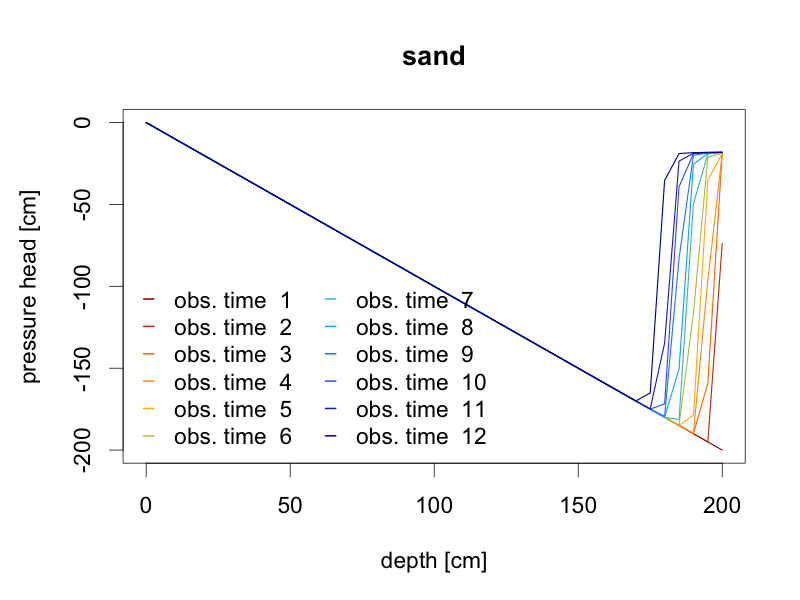
\includegraphics[width=0.49\textwidth]{Fig_inf1/obs_press_head_sand.png}
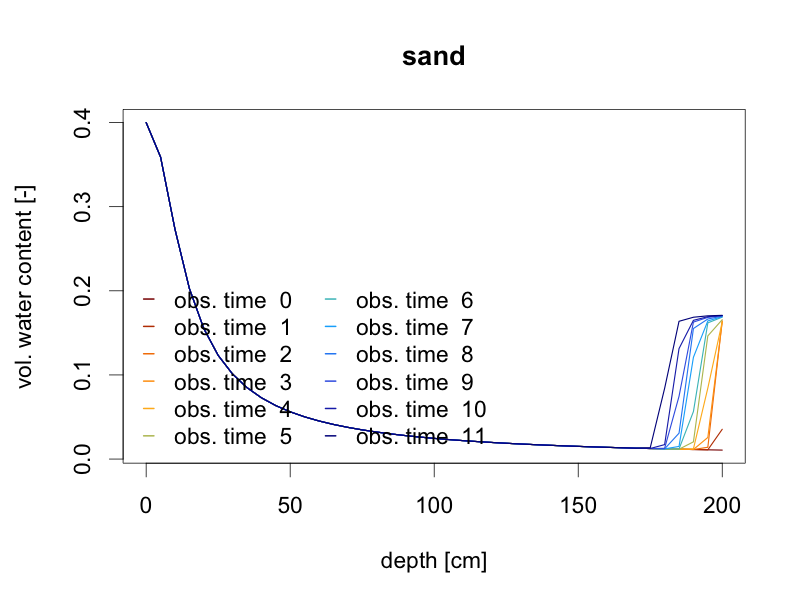
\includegraphics[width=0.49\textwidth]{Fig_inf1/obs_water_sand.png}
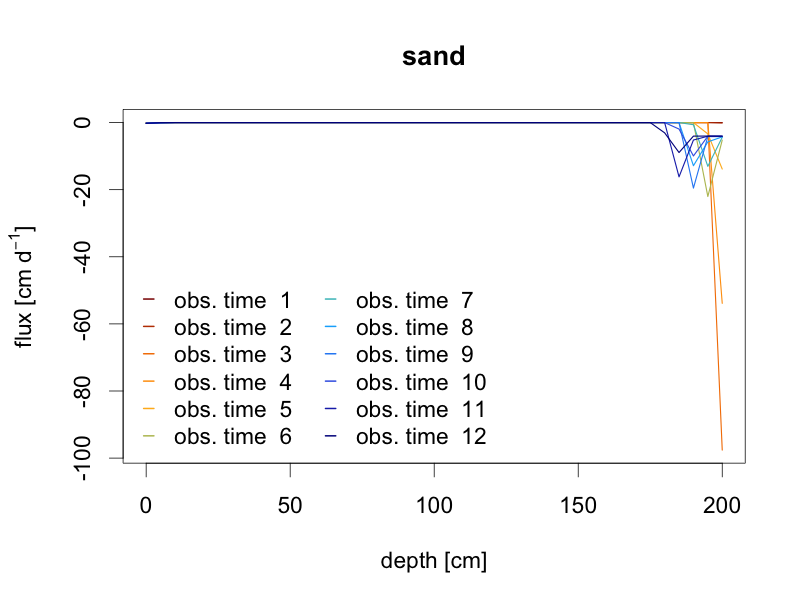
\includegraphics[width=0.49\textwidth]{Fig_inf1/obs_flux_sand.png}
\caption{Observation time series of pressure head, vol. water content and flux of infiltration into sand.}
\end{figure}

\begin{figure}
\centering
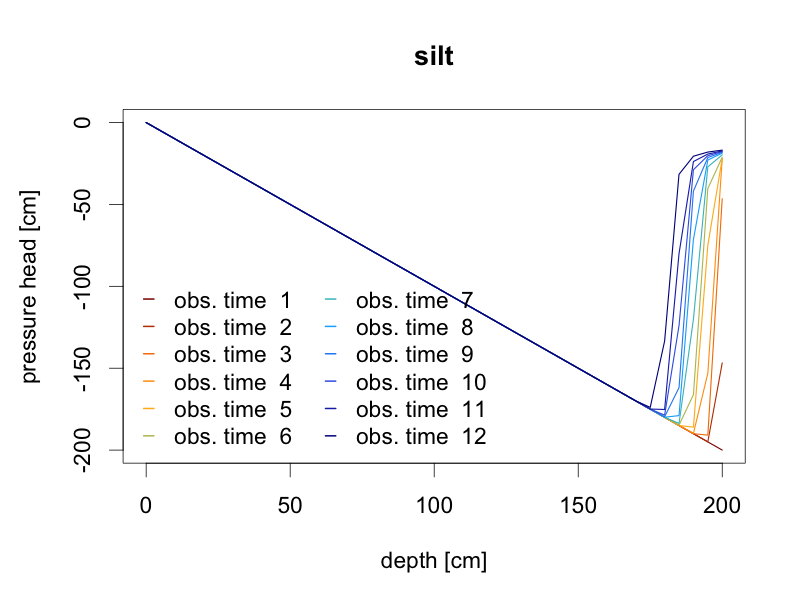
\includegraphics[width=0.49\textwidth]{Fig_inf1/obs_press_head_silt.png}
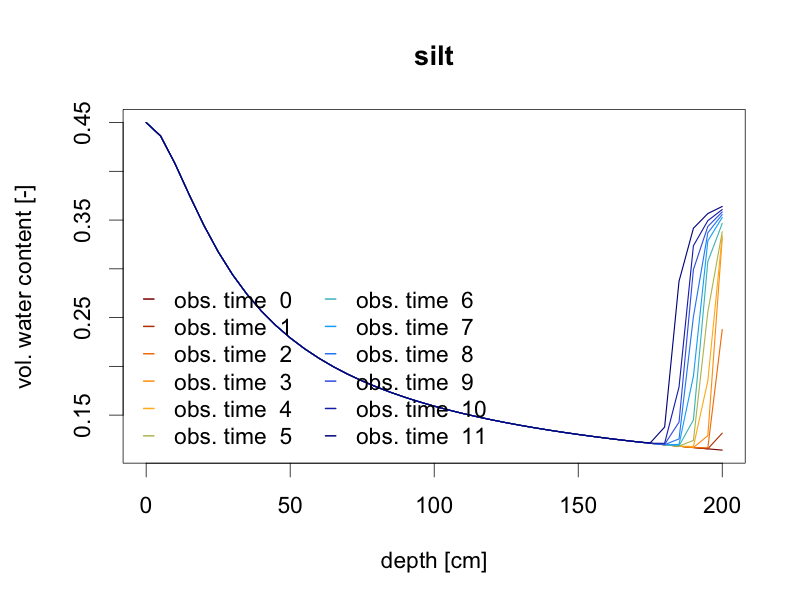
\includegraphics[width=0.49\textwidth]{Fig_inf1/obs_water_silt.png}
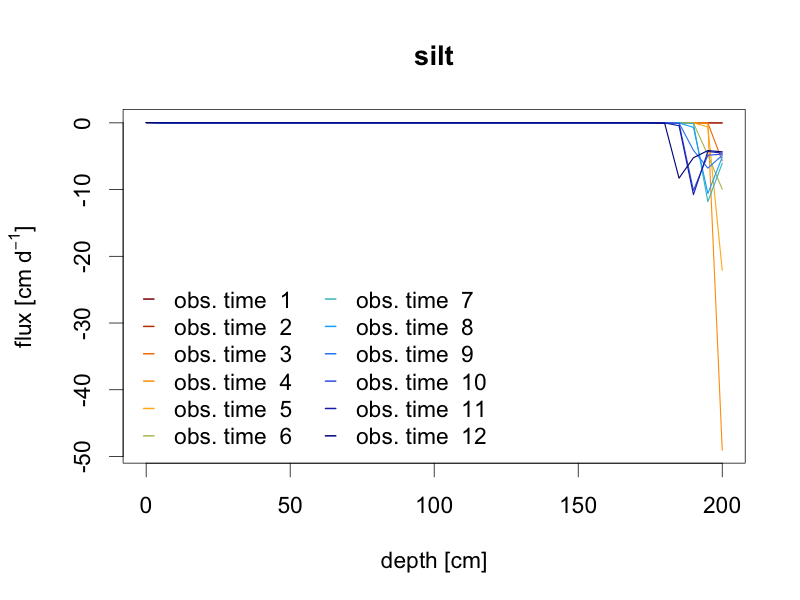
\includegraphics[width=0.49\textwidth]{Fig_inf1/obs_flux_silt.png}
\caption{Observation time series of pressure head, vol. water content and flux of infiltration into silt.}

\end{figure}


\begin{figure}
\centering
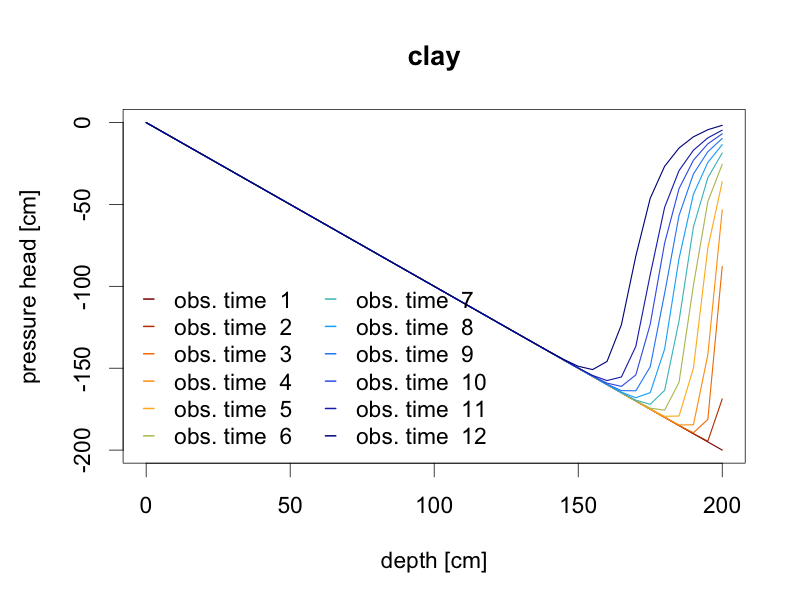
\includegraphics[width=0.49\textwidth]{Fig_inf1/obs_press_head_clay.png}
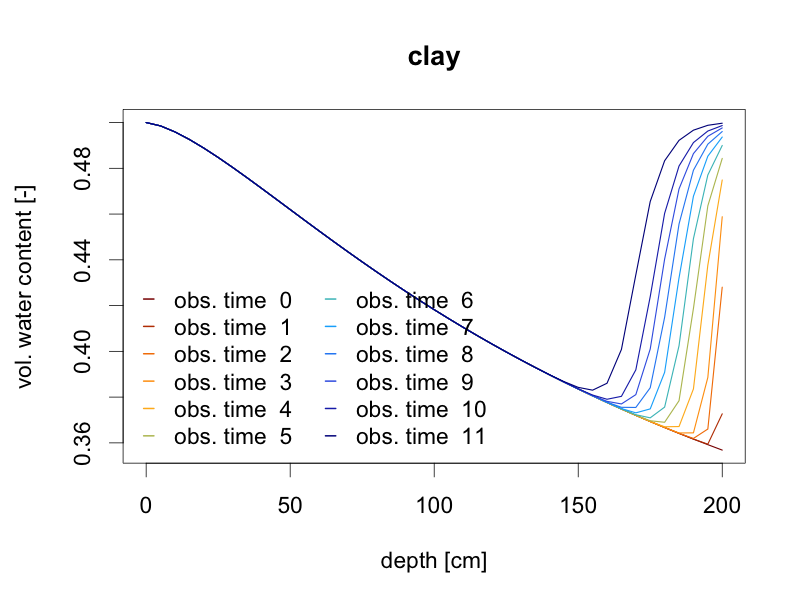
\includegraphics[width=0.49\textwidth]{Fig_inf1/obs_water_clay.png}
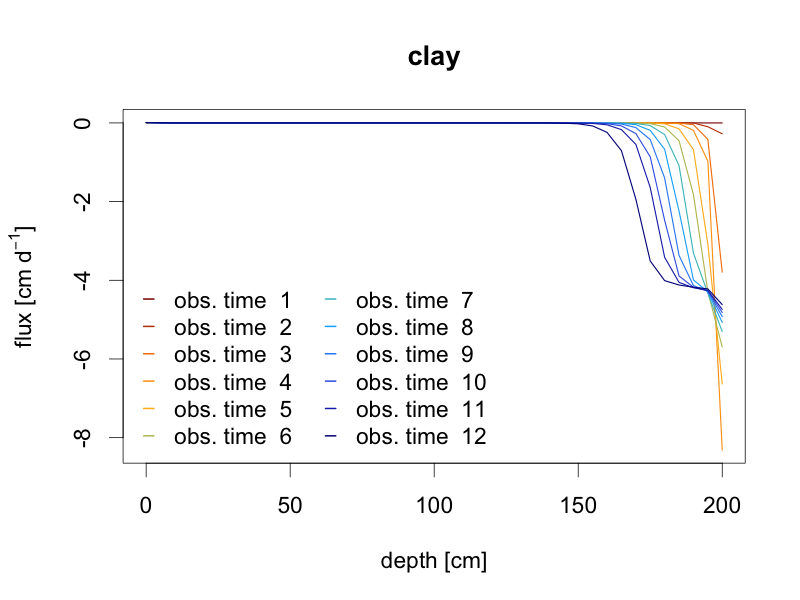
\includegraphics[width=0.49\textwidth]{Fig_inf1/obs_flux_clay.png}
\caption{Observation time series of pressure head, vol. water content and flux of infiltration into clay.}

\end{figure}

\newpage
\newpage
\newpage
\newpage
\subsection{Outcome}
\begin{enumerate}
\item You got familiar with the $DRUtES$ standard Richards Equation modules in 1D.
\item You understand basic parameterization of a typical sand, silt and clay with the van Genuchten-Mualem model.
\item You simulated infiltration in different soils.
\item You understand the term \emph{Neumann boundary condition} and \emph{initial condition}.
\item You understand the effects of different discretizations.
\end{enumerate}

\section{Infiltration - Part 2}
\subsection{Goal and Complexity}
\subsection*{Complexity: Beginner}

\subsection*{Prerequisites: None}

The goal of this tutorial is to get familiar with the $DRUtES$ standard Richards equation module and $DRUtES$ configuration in 1D by simulating infiltration into different soil \medskip

\subsection{Scenarios}

We use the same parameters as in the previous infiltration scenario (Tab. \ref{tab_inf1}). We assume a constant ponding depth at the top boundary.  Similar to the state of saturation in the previous scenario at the bottom boundary, where we knew the solution of the water table, we can assume the height of the water table, the ponding depth, to be defined with a Dirichlet condition, where the value is similar to the height of the ponding depth. At the bottom, we assume that only gravitational force acts on the bottom drainage. This also means that the pressure head gradient is zero. This boundary condition is called \textbf{free drainage}. The set-up of these scenarios are the same as in the previous infiltration scenarios, except for the boundary conditions. In these scenarios, we also want to investigate the effects on discretization, especially on the flux over the top boundary.  


\begin{figure}[!h]
\centering
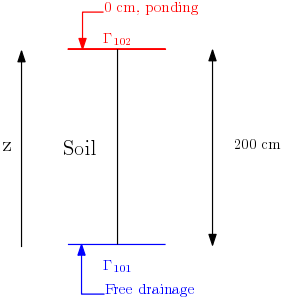
\includegraphics[width=5cm]{Fig_inf2/domain.png}
\caption{1D domain set-up of infiltration scenario with top and bottom boundary conditions. A constant ponding is assigned to the top, defined with a Dirichlet condition of 0 cm. Free drainage occurs at the bottom, which indicates that the pressure head gradient is 0 and water flows only due to gravity.}
\end{figure}

\newpage

\section*{Scenario 1}

Infiltration into sandy soil. 

$global.conf$: Choose correct model, dimension, time discretization and observation times.
\begin{enumerate}
\item Open \textbf{\emph{global.conf}} in a text editor of your choice. 
\item Model type: Your first input is the module. Input is \textbf{RE}.
\item Initial mesh configuration \begin{enumerate}
\item The dimension of our problem is 1. Input: 1.
\item We use the internal mesh generator. Input: 1. 
\end{enumerate}
\item Error criterion \begin{enumerate} 
\item Maximum number of iteration of the Picard method: 20 
\item h tolerance: 1e-1.
\end{enumerate}
\item Time information 
\begin{enumerate} 
%\item integration method is 3 point formula. Input: 30. 
\item Time units are in hours: input d
\item Initial time: 1e-4.
\item End time: 1.
\item Minimum time step: 1e-4.
\item Maximum time step: 0.1.
\end{enumerate}
\item Observation time settings \begin{enumerate}
\item Observation time method: 2
\item Set file format of observation: pure. Output in 1D is always in raw data. Different options will not impact output in 1D.
\item Make sequence of observation time: n
\item Number of observation times: 10
\item Observation time values: 0.001,
0.005,
0.01,
0.05,
0.1,
0.2,
0.3,
0.4,
0.6,
0.8. Use a new line for each input. \textit{DRUtES} automatically generates output for the initial time and final time. DRUtES will generate 12 output files, e.g. \textit{RE\_matrix\_press\_head-x.dat}, \textit{RE\_matrix\_theta-x.dat} where x is the number of the file and not the output time. The initial time is assigned an x value of 0. 
\end{enumerate}
\item Observation point settings \begin{enumerate}
\item Observation point coordinates: 0, 200. Use a new line for each input. \textit{DRUtES} will generate 2 output files, e.g. \textit{obspt\_RE\_matrix-1.out}, where x is the ID of the observation point. 
\end{enumerate}
\item Ignore other settings for now. 
\item Save $global.conf$
\end{enumerate}


$drumesh1D.conf$: Mesh definition, i.e. number of materials and spatial discretization
\begin{enumerate}
\item Open \textbf{\emph{drumesh1D.conf}} in a text editor of your choice. 
\item Geometry information: 200 cm - domain length
\item Amount of intervals: 1
\item
\adjustbox{max height=\dimexpr\textheight-5cm\relax,
           max width=\textwidth}{
\small\begin{tabular}{|c | c | c|}
\hline
density & bottom & top \\
 \hline
5 & 0 & 200\\
\hline
\end{tabular}
}
\item number of materials: 1
\item \adjustbox{max height=\dimexpr\textheight-5cm\relax,
           max width=\textwidth}{
\small\begin{tabular}{|c | c | c|}
\hline
id & bottom & top \\
 \hline
5 & 0 & 200 \\
\hline
\end{tabular}
}
\end{enumerate}

\emph{matrix.conf}: Configuration file for water flow 


\begin{enumerate}
\item Open \emph{matrix.conf} in a text editor of your choice. 
\item How-to use constitutive relations? [integer]: 1
\item Length of interval for precalculating the constitutive functions: 200
\item Discretization step for constituitive function precalculation: 0.1
\item number of soil layers [integer]: 1
\item \adjustbox{max height=\dimexpr\textheight-5cm\relax,
	max width=\textwidth}{
	\small\begin{tabular}{|c | c | c|c | c | c|}
		\hline
		alpha & n & m & theta\_r & theta\_s & specific storage\\
		\hline
		0.1 & 2.2  & 0.55 & 0.00 & 0.40  &0  \\
		\hline
	\end{tabular}
}
\item The angle of the anisotropy determines the angle of the reference coordinate system. 0 means vertical flow. Anisotropy description. Anisotpropy description and hydraulic conductivity\\ \adjustbox{max height=\dimexpr\textheight-5cm\relax,
	max width=\textwidth}{
	\small\begin{tabular}{|c | c |}
		\hline
		angle [degrees] & K\_11  \\
		\hline
		0 & 400  \\
		\hline
	\end{tabular}
}
\item sink(-) /source (+) term per layer: 0
\item Initial condition is a constant pressure head of -200 cm across the soil. \\ \adjustbox{max height=\dimexpr\textheight-5cm\relax,
	max width=\textwidth}{
	\small\begin{tabular}{|c | c | c|c |}
		\hline
		 init. cond [real] & type of init. cond &RCZA method [y/n] &  RCZA method val.  \\
		\hline
		   -200.0           &            hpres                       & n		   &          0 \\
		\hline
	\end{tabular}
}
\item number of boundaries: 2
\item \adjustbox{max height=\dimexpr\textheight-5cm\relax,
	max width=\textwidth}{
	\small\begin{tabular}{|c | c | c|c |}
		\hline
		boundary ID& boundary type   & use rain.dat [y/n]   & value  \\
		\hline
	101    &                   3        &           n        &        0.0 \\
	102             &          1         &          n         &       0.0        \\
	
		\hline
	\end{tabular}
}
\item Save matrix.conf.

\end{enumerate}

\section*{Run scenario 1}
Run the simulation in the terminal console.
\begin{enumerate}
\item Make sure you are in the right directory. 
\item To execute $DRUtES$: \\
\$ bin/drutes
\item After the simulation finishes, to generate png plots execute provided R script: \\
\$ Rscript drutes.conf/water.conf/waterplots.R -name sand
\item The output of the simulation can be found in the folder out
\end{enumerate}

\section*{Scenario 2}
Infiltration into silty soil
\begin{enumerate}
\item \emph{global.conf} and \emph{drumesh1D.conf} remain the same.
\item Open \emph{matrix.conf} in a text editor of your choice. 
\item Use the same set-up, but change the van Genuchten parameters to:
\item \adjustbox{max height=\dimexpr\textheight-5cm\relax,
	max width=\textwidth}{
	\small\begin{tabular}{|c | c | c|c | c | c|}
		\hline
		alpha & n & m & theta\_r & theta\_s & specific storage\\
		\hline
		0.08 & 1.8   & 0.44 & 0.05 & 0.45  & 0 \\
		\hline
	\end{tabular}
}
\item anisothprophy description and hydraulic conductivity\\ \adjustbox{max height=\dimexpr\textheight-5cm\relax,
	max width=\textwidth}{
	\small\begin{tabular}{|c | c |}
		\hline
		angle [degrees] & K\_11  \\
		\hline
		0 & 40  \\
		\hline
	\end{tabular}
}
\item Save matrix.conf.
\end{enumerate}

\section*{Run scenario 2}
Run the simulation in the terminal console.
\begin{enumerate}
\item To execute $DRUtES$: \\
\$ bin/drutes
\item generate png plots with R script: \\
\$ Rscript drutes.conf/water.conf/waterplots.R -name silt
\end{enumerate}

\section*{Scenario 3}
Infiltration into clay soil
\begin{enumerate}
\item \emph{global.conf} and \emph{drumesh1D.conf} remain the same.
\item Open \emph{matrix.conf} in a text editor of your choice. 
\item Use the same set-up, but change the van Genuchten parameters to:
\item \adjustbox{max height=\dimexpr\textheight-5cm\relax,
	max width=\textwidth}{
	\small\begin{tabular}{|c | c | c|c | c | c|}
		\hline
		alpha & n & m & theta\_r & theta\_s & specific storage\\
		\hline
		0.01 & 1.5  & 0.33 & 0.1& 0.5   &0 \\
		\hline
	\end{tabular}
}
\item anisothprophy description and hydraulic conductivity\\ \adjustbox{max height=\dimexpr\textheight-5cm\relax,
	max width=\textwidth}{
	\small\begin{tabular}{|c | c |}
		\hline
		angle [degrees] & K\_11  \\
		\hline
		0 & 4  \\
		\hline
	\end{tabular}
}
\item Save matrix.conf.
\end{enumerate}

\section*{Run scenario 3}
Run the simulation in the terminal console.
\begin{enumerate}
\item To execute $DRUtES$: \\
\$ bin/drutes
\item generate png plots with R script: \\
\$ Rscript drutes.conf/water.conf/waterplots.R -name clay
\end{enumerate}

\section*{Tasks}

\begin{enumerate}
\item Describe the infiltration fronts for sand, silt and clay.
\item The results do not look very smooth. This is because of insufficient discretization. Improve the discretization for sand. With what set-up are the results better? Possibilities are: 
\begin{itemize}
\item in global.conf: Decrease the pressure head tolerance, Decrease the initial time step, Decrease the maximum time step.
\item in drumesh1D.conf: Decrease the mesh density. 
\end{itemize}
\item Why is the flux at the top so huge in the beginning?
\end{enumerate}



\section*{Results}

\subsection*{Task 1}
In the following time series of the infiltration into sand, silt and clay are presented. The infiltration front has moved furthest in sand, followed by silt and then clay. This is because of the assigned boundary conditions. The flux into sandy soil is very large. However, the time series show the numerical approximation is insufficient, especially for sand. This is because sand is the numerically most difficult to model as it has the steepest retention properties (largest n and largest alpha).

\begin{figure}[!h]
\centering
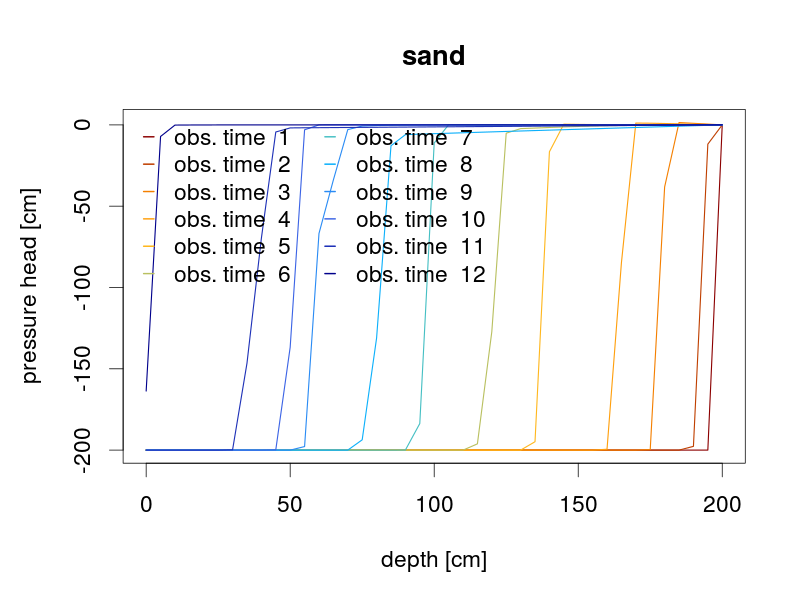
\includegraphics[width=0.49\textwidth]{Fig_inf2/obs_press_head_sand.png}
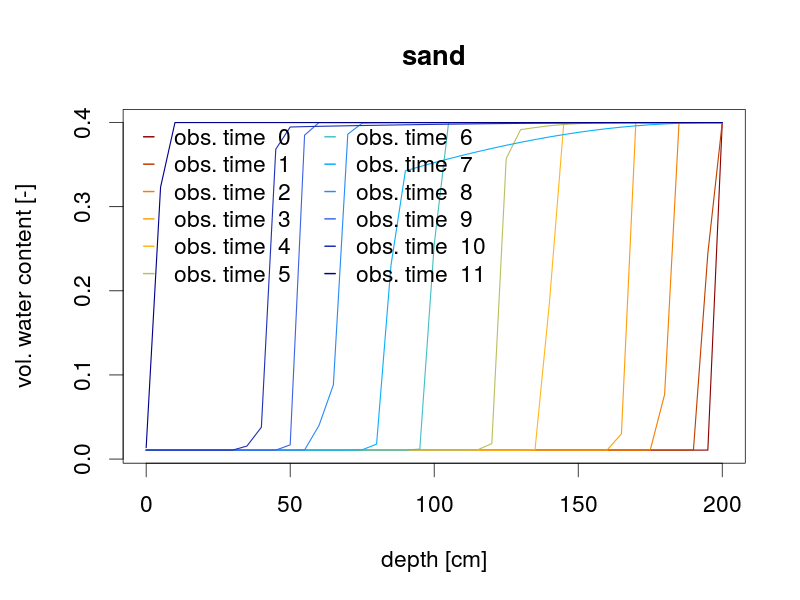
\includegraphics[width=0.49\textwidth]{Fig_inf2/obs_water_sand.png}
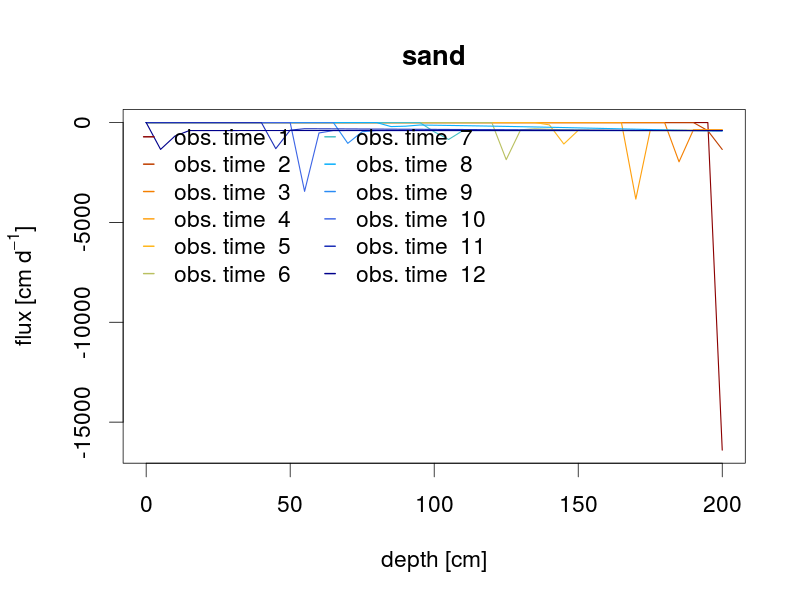
\includegraphics[width=0.49\textwidth]{Fig_inf2/obs_flux_sand.png}
\caption{Observation time series of pressure head, vol. water content and flux of infiltration into sand.}
\end{figure}

\begin{figure}[!h]
\centering
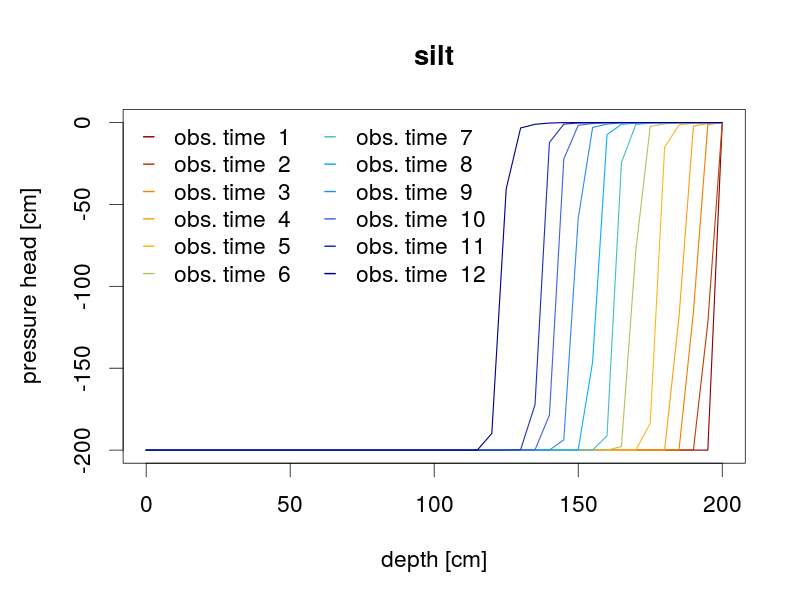
\includegraphics[width=0.49\textwidth]{Fig_inf2/obs_press_head_silt.png}
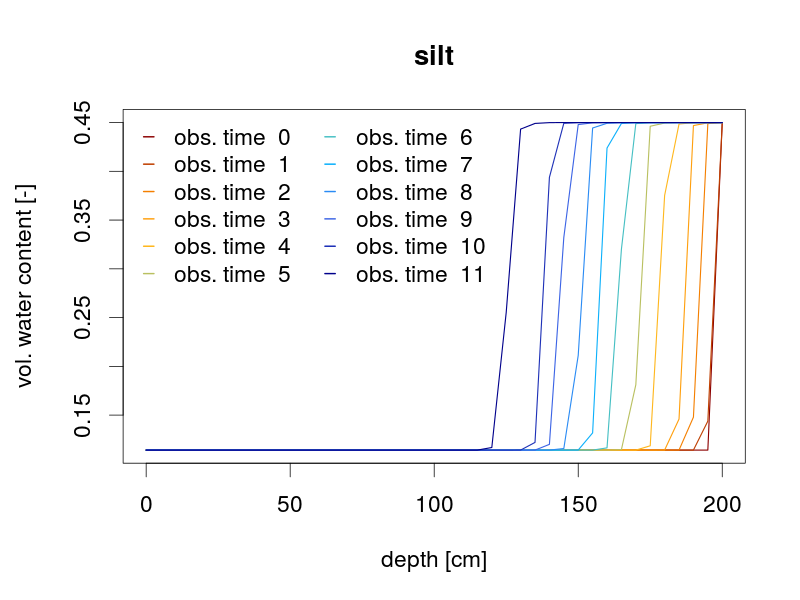
\includegraphics[width=0.49\textwidth]{Fig_inf2/obs_water_silt.png}
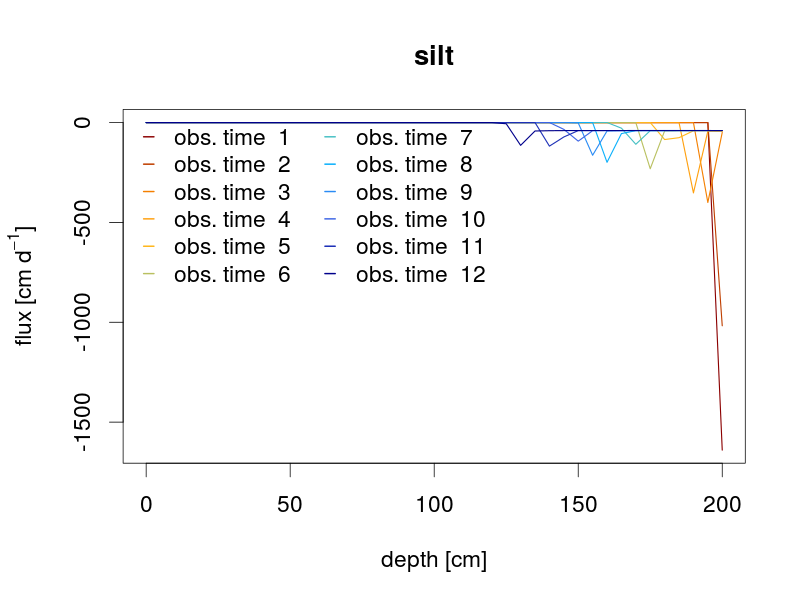
\includegraphics[width=0.49\textwidth]{Fig_inf2/obs_flux_silt.png}
\caption{Observation time series of pressure head, vol. water content and flux of infiltration into silt.}

\end{figure}


\begin{figure}[!h]
\centering
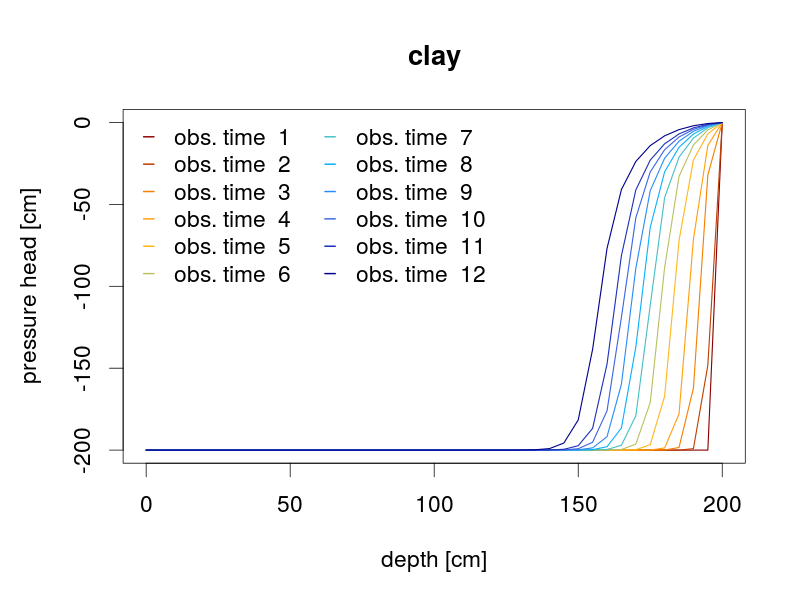
\includegraphics[width=0.49\textwidth]{Fig_inf2/obs_press_head_clay.png}
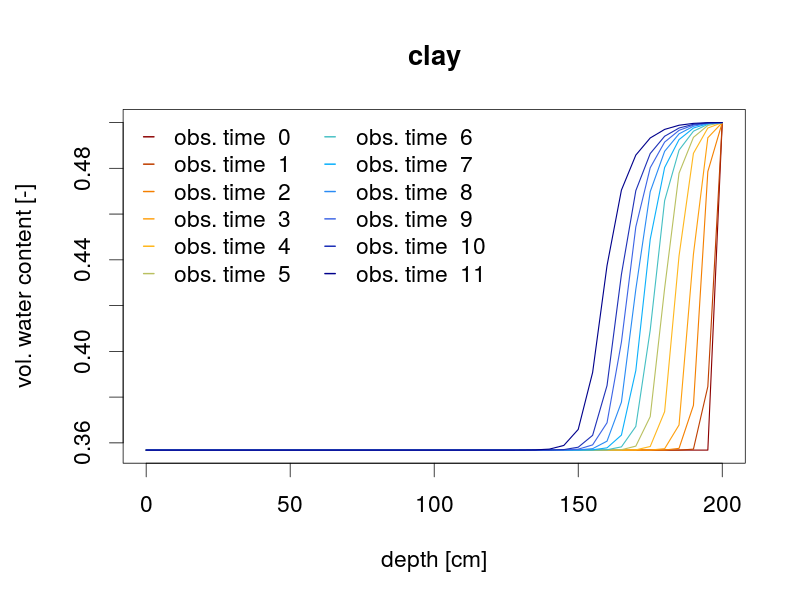
\includegraphics[width=0.49\textwidth]{Fig_inf2/obs_water_clay.png}
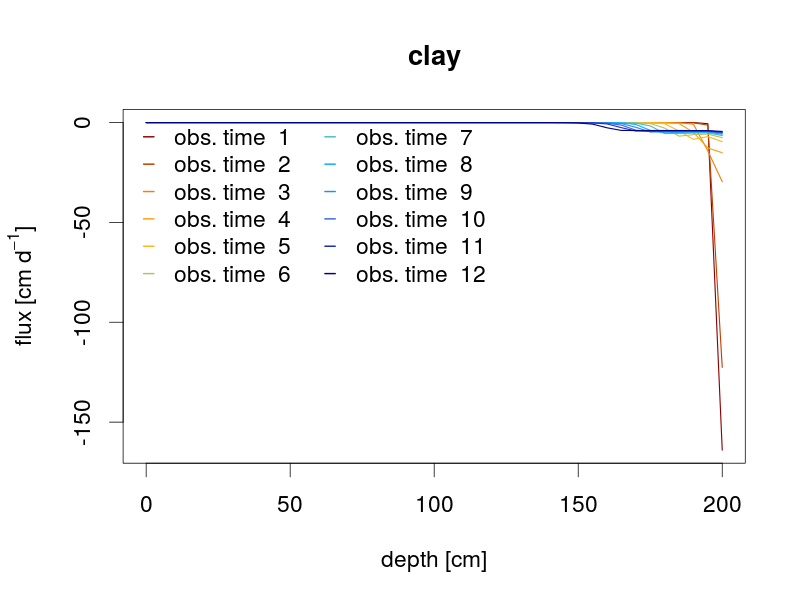
\includegraphics[width=0.49\textwidth]{Fig_inf2/obs_flux_clay.png}
\caption{Observation time series of pressure head, vol. water content and flux of infiltration into clay.}

\end{figure}

\newpage
\newpage
\subsection*{Task 2}

The solution for sand the water content and hydraulic pressure become a lot smoother with finer spatial discretization, eg. dz=0.5 and a finer temporal discretization by setting the lower minimal time step to 0.01. The fluxes are still spiky, but correlate with the infiltration front. Different solutions can be found by decreasing the minimal time step even further and also the h tolerance criterion. This, however, increases the simulation time substantially. For a reliable solution, the numerical solution should converge. This means that decreasing the time step, or discretization, should not lead to an entirely different solution. We notice, that reducing the h tolerance criterion improves the solution locally, but that reducing the maximum time step changes the depth of the infiltration front. This is because the mass balance is very much connected to the temporal discretization.

\begin{figure}[!h]
	\centering
	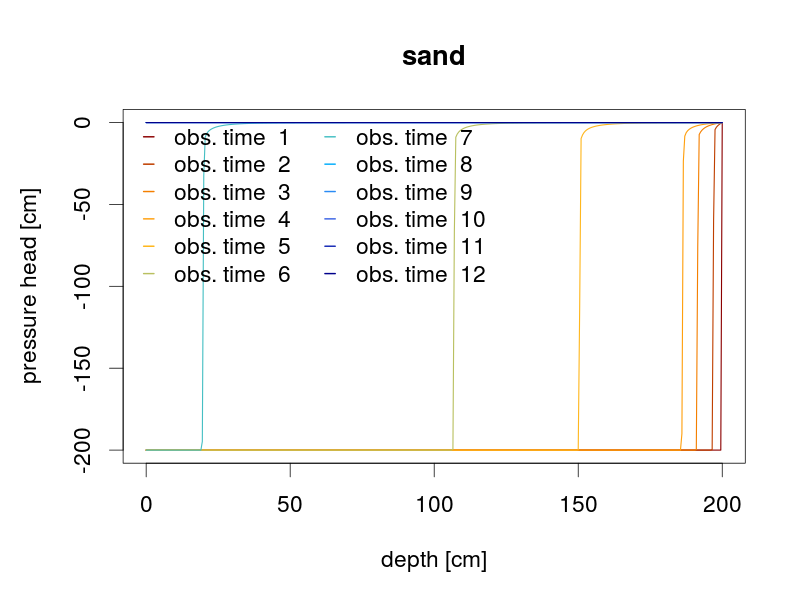
\includegraphics[width=0.49\textwidth]{Fig_inf2/obs_press_head_sand6.png}
	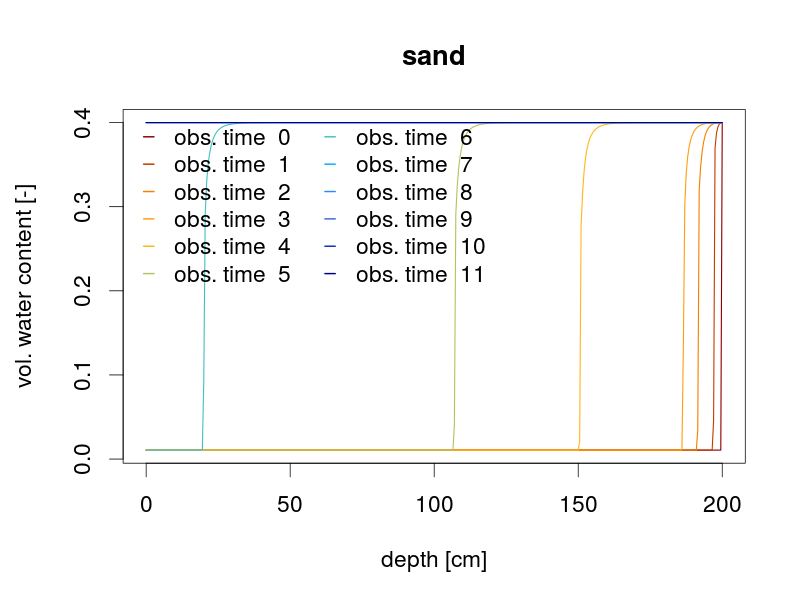
\includegraphics[width=0.49\textwidth]{Fig_inf2/obs_water_sand6.png}
	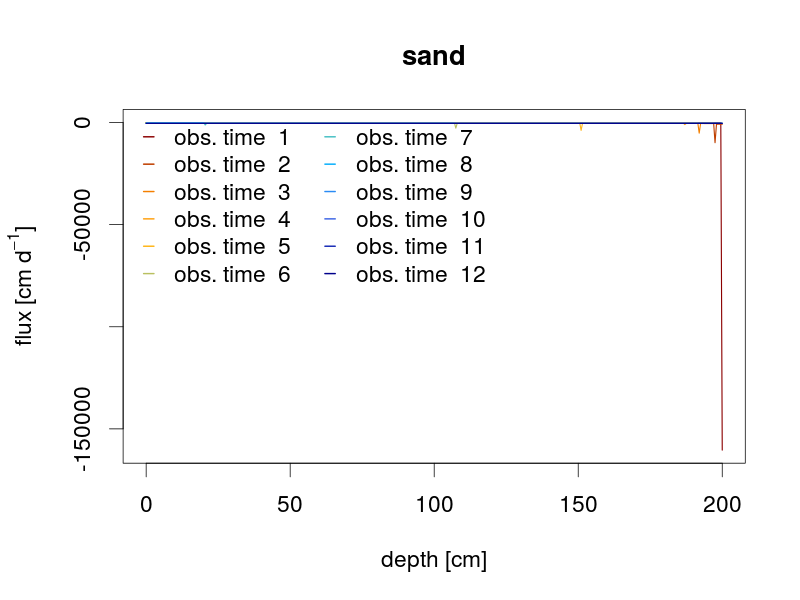
\includegraphics[width=0.49\textwidth]{Fig_inf2/obs_flux_sand6.png}
	\caption{Observation time series of pressure head, vol. water content and flux of infiltration into sand with improved discretization.}
\end{figure}

\subsection*{Task 3}
With the initial set-up, the flux at the top in sand is 15000 cm d$^{-1}$ in the beginning of the simulation. For silt, the flux was numerically calculated to be at 1500 cm d$^{-1}$ and for clay at 150 cm d$^{-1}$. The flux estimation becomes a lot larger with finer spatial discretization.

 This is due to the large hydraulic gradient between the saturated top boundary and the next node of $\nabla h=\frac{-200-0~}{\mathrm{dz}}$. The smaller the nodal distance dz is, the greater is the gradient. According to the Darcy-Buckingham law, the flux is proportional to the hydraulic conductivity. The hydraulic conductivity is highest for sand. This is why the flux is largest for sand and lowest for clay.
\newpage
\newpage
\newpage
\newpage
\subsection{Outcome}
\begin{enumerate}
\item You got familiar with the $DRUtES$ standard Richards Equation modules in 1D.
\item You understand basic parameterization of a typical sand, silt and clay with the van Genuchten-Mualem model.
\item You simulated infiltration in different soils.
\item You understand the term \emph{Free drainage} and \emph{initial condition}.
\item You understand the effects of different discretizations.
\end{enumerate}

\resetlinenumber
\chapter{Coupled models}
\section{Coupled water and heat flow}
\subsection{Goal and Complexity}
\subsection*{Complexity: Medium}

\subsection*{Prerequisites: None}

The goal of this tutorial is to get familiar with the idea of coupled models in 1D. For this we couple the $DRUtES$ standard Richards equation module and the heat module. We apply solar radiation data and rain and evaporation data as input.

\begin{figure}[!h]
\centering
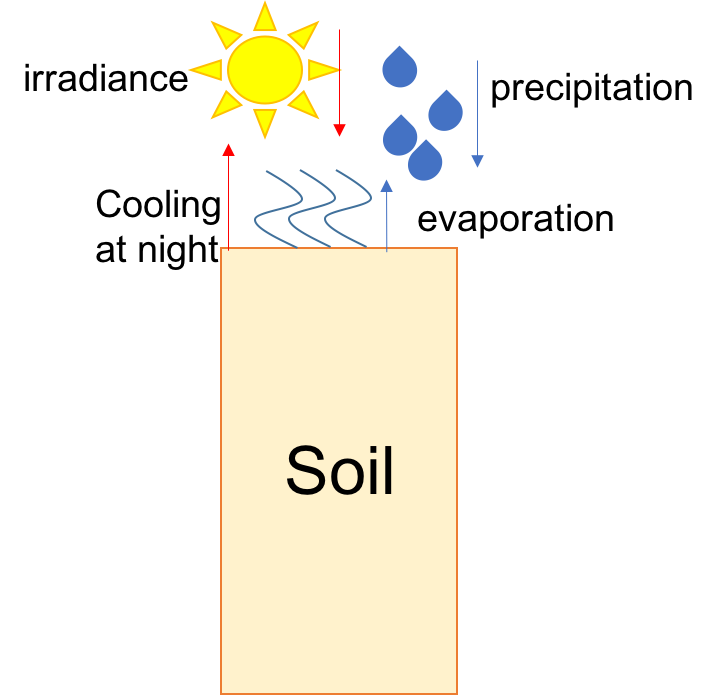
\includegraphics[width=8cm]{Fig_coupledheat/coupled.png}
\caption{Simplified scheme of coupled model.}
\end{figure}

In the real world many coupled processes occur. Heat conduction is dependent on the water content and water flow is dependent on heat properties. 

In this tutorial three configuration files will be modified step by step. All configuration files are located in the folder \emph{drutes.conf} and respective subfolders. \begin{enumerate}
\item For selection of the module, dimension and time information we require \emph{global.conf}.  \emph{global.conf} is located in \emph{drutes.conf / global.conf}. 
\item To define the mesh or spatial discretization in 1D,  we require \emph{drumesh1D.conf}. \emph{drumesh1D.conf} is located in \emph{drutes.conf / mesh / drumesh1D.conf}. 
\item To define the radiation and cooling, we require \emph{heat.conf}. \emph{heat.conf} is located in \emph{drutes.conf /heat/ heat.conf}. 
\item To define the precipitation and evaporation, we require \emph{matrix.conf}. \emph{matrix.conf} is located in \emph{drutes.conf /water.conf/ matrix.conf}. 
\end{enumerate}
$DRUtES$ works with configuration input file with the file extension .conf. Blank lines and lines starting with \# are ignored. The input mentioned in this tutorial therefore needs to be placed one line below the mentioned keyword, unless stated otherwise. 

\newpage
\subsection{Scenarios}

We are using the well-known van Genuchten-Mualem parameterization to describe the soil hydraulic properties of our soils. 

\begin{table}[!h]
\centering
\caption{\label{tab_heat}Material properties needed for scenarios.}
\adjustbox{max height=\dimexpr\textheight-2cm\relax,
           max width=\textwidth}{

\small\begin{tabular}{l l c c }
\hline
Parameter & Description & Soil \\
\hline

$\alpha$ [cm$^{-1}$]& inverse of the air entry value &0.05 \\
 $n$ [-]& shape parameter &2 \\
 $m$ [-]& shape parameter &0.5  \\
  $ \theta_s$ [-]&saturated vol. water content&0.45 \\
  $ \theta_r$ [-]& residual vol. water content&0.05  \\
  $Ss$ [cm$^{-1}$] & specific storage & 0 \\
  $K_s$ [cm d$^{-1}$] & saturated hydraulic conductivity & 100 \\ 
   $c_l$ [Wd cm$^{-3}$ K$^{-1}$ ] & specific heat capacity of soil & 2.545e-5 \\
  $c_w$ [Wd cm$^{-3}$ K$^{-1}$ ] & specific heat capacity of water & 4.843e-5	 \\ 
  $\lambda$ [W cm$^{-1}$ K$^{-1}$] & thermal conductivity & 0.02 \\ 
\hline
\end{tabular}
}
\end{table}


\begin{figure}[!h]
\centering
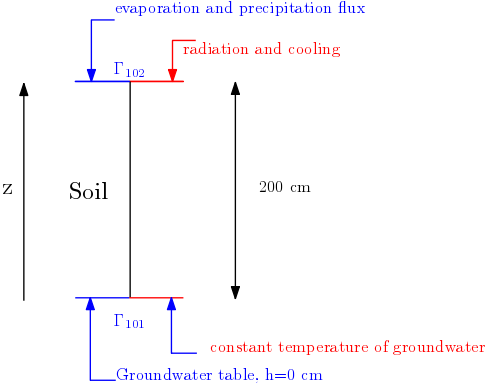
\includegraphics[width=10cm]{Fig_coupledheat/domain_coupled.png}
\caption{1D domain set-up of coupled scenario with top and bottom boundary conditions. There are now two boundary condtions at the top and two boundary conditions at the bottom: heat and water flow. The top boundary is defined by the interactions with the atmosphere and the bottom boundary is defined by the constant groundwater table.}
\end{figure}


\begin{figure}[!h]
\centering
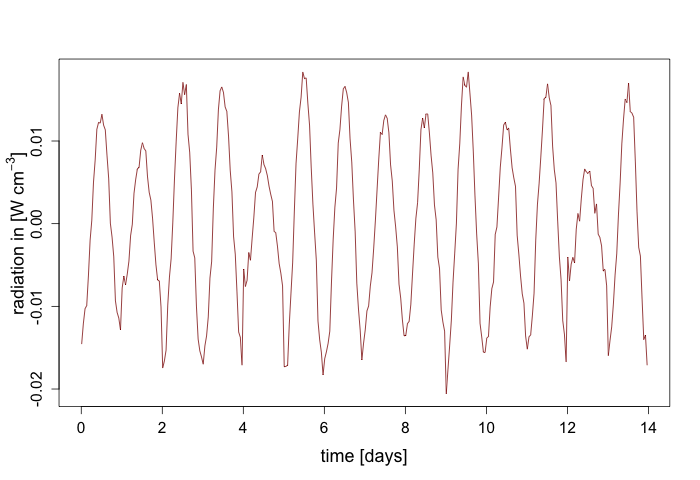
\includegraphics[width=10cm]{Fig_coupledheat/radiation_data.png}
\caption{Heat flow data used for the top boundary}
\end{figure}

\begin{figure}[!h]
\centering
\includegraphics[width=10cm]{Fig_coupledheat/water_data.png}
\caption{Water flow data used for the top boundary}
\end{figure}
\newpage

\section*{Scenario 1}

Coupled model

$global.conf$: Choose correct model, dimension, time discretization and observation times.
\begin{enumerate}
\item Open \textbf{\emph{global.conf}} in a text editor of your choice. 
\item Model type: Your first input is the module. Input is \textbf{heat}.
\item Initial mesh configuration \begin{enumerate}
\item The dimension of our problem is 1. Input: 1.
\item We use the internal mesh generator. Input: 1. 
\end{enumerate}
\item Error criterion \begin{enumerate} 
\item Maximum number of iteration of the Picard method: 20 
\item h tolerance: 1.
\end{enumerate}
\item Time information 
\begin{enumerate} 
%\item integration method is 3 point formula. Input: 30. 
\item Time units are in hours: input d
\item Initial time: 1e-6.
\item End time: 14.
\item Minimum time step: 1e-6.
\item Maximum time step: 0.001.
\end{enumerate}
\item Observation time settings \begin{enumerate}
\item Observation time method: 2
\item Set file format of observation: pure. Output in 1D is always in raw data. Different options will not impact output in 1D.
\item Make sequence of observation time: n
\item Number of observation times: 0
\item Observation time values: \#
\end{enumerate}
\item Observation point settings \begin{enumerate}
\item Number of observation points: 6 
\item Observation point coordinates: 200, 195,180,160,140, 120. Use a new line for each input. \textit{DRUtES} will generate 6 output files, e.g. \textit{obspt\_RE\_matrix-1.out}, where x is the ID of the observation point. 
\end{enumerate}
\item Ignore other settings for now. 
\item Save $global.conf$
\end{enumerate}


$drumesh1D.conf$: Mesh definition, i.e. number of materials and spatial discretization
\begin{enumerate}
\item Open \textbf{\emph{drumesh1D.conf}} in a text editor of your choice. 
\item Geometry information: 200 cm - domain length
\item Amount of intervals: 1
\item
\adjustbox{max height=\dimexpr\textheight-5cm\relax,
           max width=\textwidth}{
\small\begin{tabular}{|c | c | c|}
\hline
density & bottom & top \\
 \hline
4 & 0 & 200\\
\hline
\end{tabular}
}
\item number of materials: 1
\item \adjustbox{max height=\dimexpr\textheight-5cm\relax,
           max width=\textwidth}{
\small\begin{tabular}{|c | c | c|}
\hline
id & bottom & top \\
 \hline
1 & 0 & 200 \\
\hline
\end{tabular}
}
\end{enumerate}

\emph{matrix.conf}: Configuration file for water flow 


\begin{enumerate}
\item Open \emph{matrix.conf} in a text editor of your choice. 
\item How-to use constitutive relations? [integer]: 1
\item Length of interval for precalculating the constitutive functions: 200
\item Discretization step for constituitive function precalculation: 0.1
\item number of soil layers [integer]: 1
\item \adjustbox{max height=\dimexpr\textheight-5cm\relax,
	max width=\textwidth}{
	\small\begin{tabular}{|c | c | c|c | c | c|}
		\hline
		alpha & n & m & theta\_r & theta\_s & specific storage\\
		\hline
		0.05 & 2  & 0.5 & 0.05 & 0.45  &0  \\
		\hline
	\end{tabular}
}
\item The angle of the anisotropy determines the angle of the reference coordinate system. 0 means vertical flow. Anisotropy description. Anisotpropy description and hydraulic conductivity\\ \adjustbox{max height=\dimexpr\textheight-5cm\relax,
	max width=\textwidth}{
	\small\begin{tabular}{|c | c |}
		\hline
		angle [degrees] & K\_11  \\
		\hline
		0 & 100  \\
		\hline
	\end{tabular}
}
\item sink(-) /source (+) term per layer: 0
\item Initial condition is a constant pressure head of -200 cm across the soil. \adjustbox{max height=\dimexpr\textheight-5cm\relax,
	max width=\textwidth}{
	\small\begin{tabular}{|c | c | c|c |}
		\hline
		 init. cond [real] & type of init. cond &RCZA method [y/n] &  RCZA method val.  \\
		\hline
		   0.0           &            H\_tot                      & n		   &          0 \\
		\hline
	\end{tabular}
}
\item number of boundaries: 2
\item \adjustbox{max height=\dimexpr\textheight-5cm\relax,
	max width=\textwidth}{
	\small\begin{tabular}{|c | c | c|c |}
		\hline
		boundary ID& boundary type   & use rain.dat [y/n]   & value  \\
		\hline
	101    &                   1        &           n        &        0.0 \\
	102             &          2         &          y         &       0.0        \\
	
		\hline
	\end{tabular}
}
\item Save matrix.conf.
\end{enumerate}

\emph{heat.conf}: Heat module after Sophocleous (1979). 


\begin{enumerate}
\item Open \emph{heat.conf} in a text editor of your choice. 

\item Couple with Richards equation: y
\item Number of materials or layers: 1 
\item Specific heat capacity of the wall material:  2.545e-5 Wd cm$^{-3}$ K$^{-1}$ 
\item Specific heat capacity of liquid: 4.843e-5  Wd cm$^{-3}$ K$^{-1}$ 
\item Anisotropy: There is no anisotropy. The value is 0.
\item Heat conductivity of the soil material: 0.02 W cm$^{-1}$ K$^{-1}$. 
\item There is NO heat convection of water: 0.
\item The initial temperature is 0$^{\circ}$C across the entire domain: 0.
\item There is no heat source: 0. 
\item We have 2 boundaries at top and bottom of the soil column. We assume a constant temperature of 15 $^{\circ}$C at the bottom where the groundwater table is. We assume the the top to be influenced by radiation and cooling, which are both flux or Neumann conditions. \\
\adjustbox{max height=\dimexpr\textheight-5cm\relax,
           max width=\textwidth}{
\small\begin{tabular}{|c | c | c| c|}
\hline
boundary id & boundary type & use bc.dat & value \\
 \hline
101& 1 & n & 15.0 \\
102& 2 & y & 0.0 \\
\hline
\end{tabular}
}

\item Save heat.conf.
\end{enumerate}

\section*{Run scenario 1}
Run the simulation in the terminal console.
\begin{enumerate}
\item Make sure you are in the right directory. 
\item To execute $DRUtES$: \\
\$ bin/drutes
\item After the simulation finishes, to generate png plots execute provided R script: \\
\$ Rscript drutes.conf/water.conf/waterplots.R -name coupled \\
\$ Rscript drutes.conf/heat/heatplots.R coupled
\item The output of the simulation can be found in the folder out
\end{enumerate}


\section*{Tasks}

\begin{enumerate}
\item Describe the temperature and water content distribution.
\end{enumerate}



\section*{Results}

The water content at the top follows the flux input. The lower the observation point, the less fluctuations can be observed.
The temperature follows the heat flux input. The temperature fluctuations become smaller with depth, but also show a lag time.

\begin{figure}[!h]
\centering
\includegraphics[width=10cm]{Fig_coupledheat/obs_water_point_coupled_standard.png}
\caption{Water content at the observation points}
\end{figure}

\begin{figure}[!h]
\centering
\includegraphics[width=10cm]{Fig_coupledheat/obs_temp_point_temp_coupled_standard.png}
\caption{Temperature at the observation points.}
\end{figure}

\newpage
\newpage

\subsection{Outcome}
\begin{enumerate}
\item You got familiar with the idea of coupled models. 
\item You simulated coupled water flow and heat flow.
\item You understand the influence of distance to input flux and how the top is the most varying layer.
\end{enumerate}

\section{Coupled water flow and contaminant transport}
%----------------------------------------------------------------------------------------
%	INTRODUCTION
%----------------------------------------------------------------------------------------
\subsection{Goal and Complexity}
\subsection*{Complexity: Medium}

\subsection*{Prerequisites: Water flow module}

The goal of this tutorial is to introduce contaminant transport. For this we couple the $DRUtES$ standard Richards equation module with the ADE module. ADE stands for Advection-Dispersion-Equation. The advection will be calculated through the Richards-Equation (water flow).

\begin{figure}[!h]
\centering
\includegraphics[width=8cm]{Fig_coupledade/coupled.png}
\caption{Simplified scheme of coupled model.}
\end{figure}

In this example we assume that the contaminant is soluble and in the water. No adsorption or desorption occurs. 

In this tutorial five configuration files will be modified step by step. All configuration files are located in the folder \emph{drutes.conf} and respective subfolders. \begin{enumerate}
\item For selection of the module, dimension and time information we require \emph{global.conf}.  \emph{global.conf} is located in \emph{drutes.conf / global.conf}. 
\item To define the mesh or spatial discretization in 1D,  we require \emph{drumesh1D.conf}. \emph{drumesh1D.conf} is located in \emph{drutes.conf / mesh / drumesh1D.conf}. 
\item To define the precipitation, we require \emph{matrix.conf}. \emph{matrix.conf} is located in \emph{drutes.conf /water.conf/ matrix.conf}. 
\item To select the ADE module and link it to the water module, we require \emph{ADE.conf}. \emph{ADE.conf} is located in \emph{drutes.conf /ADE/ ADE.conf}. 
\item To define the contaminant transport, we require \emph{contaminant.conf}. \emph{contaminant.conf} is located in \emph{drutes.conf /ADE/ contaminant.conf}. 
\end{enumerate}
$DRUtES$ works with configuration input file with the file extension .conf. Blank lines and lines starting with \# are ignored. The input mentioned in this tutorial therefore needs to be placed one line below the mentioned keyword, unless stated otherwise. 

\newpage
\subsection{Scenarios}

In the following scenario, there is a contaminant of a known concentration in the soil, which we can set with appropriate layering of our domain and the initial condition. This coupled model also requires four boundary conditions, two for the water flow and two for the contaminant transport. We assume that the contaminant does not reach the bottom of our domain, nor the top boundary. The boundary conditions for the contaminant transport at both boundaries are constant Dirichlet conditions. The bottom boundary represents the groundwater table. We assign a Dirichlet condition for the water flow at the bottom of the profile. We assume precipitation occurs at the top boundary and therefore, we assign a Neumann condition at the top boundary. In these scenarios we want to investigate the effect of a soil layer with different hydraulic properties below the contaminant.  

\begin{table}[!h]
\centering
\caption{\label{tab_coup2}Material properties needed for scenarios.}
\adjustbox{max height=\dimexpr\textheight-2cm\relax,
           max width=\textwidth}{

\small\begin{tabular}{l l c c c }
\hline
Parameter & Description & Sand & Clay & Contaminant\\
\hline

$\alpha$ [cm$^{-1}$]& inverse of the air entry value &0.05 & 0.01 \\
 $n$ [-]& shape parameter &2 & 1.4\\
 $m$ [-]& shape parameter &0.5 & 0.2857  \\
  $ \theta_s$ [-]&saturated vol. water content&0.45 &0.45 \\
  $ \theta_r$ [-]& residual vol. water content&0.05 &0.05  \\
  $Ss$ [cm$^{-1}$] & specific storage & 0 & 0 \\
  $K_s$ [cm d$^{-1}$] & saturated hydraulic conductivity & 100 & 1\\ 
  D [cm$^{2}$ d$^{-1}$] & diffusion  &10e-3& 10e-3 \\
  D$_v$ [cm ] & dispersivity  & 30 & 100	 \\ 
 c$_\mathrm{init}$ [mg cm$^{-3}$] & initial concentration & & & 2\\
\hline
\end{tabular}
}
\end{table}

The domain scheme is shown in Fig. \ref{domain}. We need to define 4 boundary conditions. Our mesh requires 5 different layers to accomodate for the contaminantion, the extra soil and the layers in between.

\begin{figure}[!h]
\centering
\includegraphics[width=10cm]{Fig_coupledade/domain_set_upADEwater.png}
\caption{\label{domain}1D domain set-up of coupled scenario with top and bottom boundary conditions. There are now two boundary condtions at the top and two boundary conditions at the bottom: contaminant transport and water flow. The top boundary is defined by the interactions with the atmosphere and the bottom boundary is defined by the constant groundwater table.}
\end{figure}

\section*{Scenario 1}

We first assume that the soil is homogeneous.

$global.conf$: Choose correct model, dimension, time discretization and observation times.
\begin{enumerate}
\item Open \textbf{\emph{global.conf}} in a text editor of your choice. 
\item Model type: Your first input is the module. Input is \textbf{ADE}.
\item Initial mesh configuration \begin{enumerate}
\item The dimension of our problem is 1. Input: 1.
\item We use the internal mesh generator. Input: 1. 
\end{enumerate}
\item Error criterion \begin{enumerate} 
\item Maximum number of iteration of the Picard method: 20 
\item h tolerance: 1e-3.
\end{enumerate}
\item Time information 
\begin{enumerate} 
%\item integration method is 3 point formula. Input: 30. 
\item Time units are in hours: input d
\item Initial time: 1e-4.
\item End time: 10.
\item Minimum time step: 1e-12.
\item Maximum time step: 0.005.
\end{enumerate}
\item Observation time settings \begin{enumerate}
\item Observation time method: 2
\item Set file format of observation: pure. Output in 1D is always in raw data. Different options will not impact output in 1D.
\item Make sequence of observation time: n
\item Number of observation times: 9
\item Observation time values: 1, 2, 3,4,5,6,7,8,9. Use a new line for each input. \textit{DRUtES} will generate 11 output files for each modeled component, e.g.\textit{RE\_matrix\_press\_head-x.dat}, where x is the ID of the observation point. The initial and final time value will be automatically be printed.
\end{enumerate}
\item Observation point settings \begin{enumerate}
\item Number of observation points: 6 
\item Observation point coordinates: 200, 195,187.5,182.5,175, 150. Use a new line for each input. \textit{DRUtES} will generate 6 output files for each modeled component, e.g. \textit{obspt\_RE\_matrix-1.out}, where x is the ID of the observation point. 
\end{enumerate}
\item Ignore other settings for now. 
\item Save $global.conf$
\end{enumerate}


$drumesh1D.conf$: Mesh definition, i.e. number of materials and spatial discretization
\begin{enumerate}
\item Open \textbf{\emph{drumesh1D.conf}} in a text editor of your choice. 
\item Geometry information: 200 cm - domain length
\item Amount of intervals: 1
\item
\adjustbox{max height=\dimexpr\textheight-5cm\relax,
           max width=\textwidth}{
\small\begin{tabular}{|c | c | c|}
\hline
density & bottom & top \\
 \hline
4 & 0 & 200\\
\hline
\end{tabular}
}
\item number of materials: 5
\item \adjustbox{max height=\dimexpr\textheight-5cm\relax,
           max width=\textwidth}{
\small\begin{tabular}{|c | c | c|}
\hline
id & bottom & top \\
 \hline
1   &     0         & 170 \\
2   &     170      &  180 \\
3   &     180     &   185 \\
4    &    185     &   190 \\
5    &    190    &    200 \\
\hline
\end{tabular}
}
\item Save $drumesh1D.conf$
\end{enumerate}

\emph{matrix.conf}: Configuration file for water flow 


\begin{enumerate}
\item Open \emph{matrix.conf} in a text editor of your choice. 
\item How-to use constitutive relations? [integer]: 1
\item Length of interval for precalculating the constitutive functions: 200
\item Discretization step for constituitive function precalculation: 0.1
\item number of soil layers [integer]: 5
\item \adjustbox{max height=\dimexpr\textheight-5cm\relax,
	max width=\textwidth}{
	\small\begin{tabular}{|c | c | c|c | c | c|}
		\hline
		alpha & n & m & theta\_r & theta\_s & specific storage\\
		\hline
		0.05 & 2  & 0.5 & 0.05 & 0.45  &0  \\
			0.05 & 2  & 0.5 & 0.05 & 0.45  &0  \\
				0.05 & 2  & 0.5 & 0.05 & 0.45  &0  \\
					0.05 & 2  & 0.5 & 0.05 & 0.45  &0  \\
						0.05 & 2  & 0.5 & 0.05 & 0.45  &0  \\
		\hline
	\end{tabular}
}
\item The angle of the anisotropy determines the angle of the reference coordinate system. 0 means vertical flow. Anisotropy description. Anisotpropy description and hydraulic conductivity\\ \adjustbox{max height=\dimexpr\textheight-5cm\relax,
	max width=\textwidth}{
	\small\begin{tabular}{|c | c |}
		\hline
		angle [degrees] & K\_11  \\
		\hline
		0 & 100  \\
		0 & 100  \\
		0 & 100  \\
		0 & 100  \\
		0 & 100  \\
		\hline
	\end{tabular}
}
\item sink(-) /source (+) term per layer: \\ 0 \\ 0 \\0 \\0 \\ 0
\item Initial condition is a constant pressure head of -200 cm across the soil.\\ \adjustbox{max height=\dimexpr\textheight-5cm\relax,
	max width=\textwidth}{
	\small\begin{tabular}{|c | c | c|c |}
		\hline
		 init. cond [real] & type of init. cond &RCZA method [y/n] &  RCZA method val.  \\
		\hline
		   0.0           &            H\_tot                      & n		   &          0 \\
		   		   0.0           &            H\_tot                      & n		   &          0 \\
		   		   		   0.0           &            H\_tot                      & n		   &          0 \\
		   		   		   		   0.0           &            H\_tot                      & n		   &          0 \\
		   		   		   		   		   0.0           &            H\_tot                      & n		   &          0 \\
		\hline
	\end{tabular}
}
\item number of boundaries: 2
\item \adjustbox{max height=\dimexpr\textheight-5cm\relax,
	max width=\textwidth}{
	\small\begin{tabular}{|c | c | c|c |}
		\hline
		boundary ID& boundary type   & use rain.dat [y/n]   & value  \\
		\hline
	101    &                   1        &           n        &        0.0 \\
	102             &          2         &          n         &       0.5        \\
	
		\hline
	\end{tabular}
}
\item Save matrix.conf.
\end{enumerate}

Contaminant transport 
\emph{ADE.conf}

\begin{enumerate}
\item Open \emph{ADE.conf} in a text editor of your choice. 
\item specify coupling with Richards equation [y/n]: y
\item use sorption: n 
\item Save ADE.conf.
\end{enumerate}

\emph{contaminant.conf}

\begin{enumerate}
	\item Open \emph{contaminant.conf} in a text editor of your choice. 
	\item number of layers: 5
	\item molecular diffusion: \\ 10e-3 \\ 10e-3 \\ 10e-3 \\ 10e-3 \\ 10e-3
	\item dispersivity: \\ \adjustbox{max height=\dimexpr\textheight-5cm\relax,
		max width=\textwidth}{
		\small\begin{tabular}{|c | c |}
			\hline
			angle [degrees] & D\_11  \\
			\hline
			0 & 30  \\
			0 & 30  \\
			0 & 30  \\
			0 & 30  \\
			0 & 30  \\
			\hline
		\end{tabular}
	}
	\item initial condition: \\ \adjustbox{max height=\dimexpr\textheight-5cm\relax,
		max width=\textwidth}{
		\small\begin{tabular}{|c | c |}
			\hline
			value & type  \\
			\hline
			0 & ca  \\
			0 & ca  \\
			0 & ca  \\
			2 & ca  \\
			0 & ca  \\
			\hline
		\end{tabular}
	}
	\item number of different orders of reactions: 1
	\item orders of reaction: \\ 1 \\ 1 \\ 1 \\ 1 \\ 1
	\item reaction coefficients: \\0 \\0\\0\\0\\0 
	\item number of boundaries: 2
	\item \adjustbox{max height=\dimexpr\textheight-5cm\relax,
		max width=\textwidth}{
		\small\begin{tabular}{|c | c | c|c |}
			\hline
			boundary ID& boundary type   & use rain.dat [y/n]   & value  \\
			\hline
			101    &                   1        &           n        &        0.0 \\
			102             &          2         &          n         &       0.0        \\
			
			\hline
		\end{tabular}
	}
\item save $contaminant.conf$
\end{enumerate}

\section*{Run scenario 1}
Run the simulation in the terminal console.
\begin{enumerate}
\item Make sure you are in the right directory. 
\item To execute $DRUtES$: \\
\$ bin/drutes
\item After the simulation finishes, to generate png plots execute provided R script: \\
\$ Rscript drutes.conf/makeplot.R -name coupled\_samesoil \\
\item The output of the simulation can be found in the folder out
\end{enumerate}

\section*{Scenario 2}

In scenario 2 we introduce a clay layer in depth 170-180 cm. For this, we need to change matrix.conf and contaminant.conf. \\

Changes in matrix.conf 

\begin{enumerate}
	\item Change the 2nd van Genuchten parameter set: \\ \adjustbox{max height=\dimexpr\textheight-5cm\relax,
		max width=\textwidth}{
		\small\begin{tabular}{|c | c | c|c | c | c|}
			\hline
			alpha & n & m & theta\_r & theta\_s & specific storage\\
			\hline
			0.05 & 2  & 0.5 & 0.05 & 0.45  &0  \\
			0.01 & 1.4  & 0.2857 & 0.05 & 0.45  &0  \\
			0.05 & 2  & 0.5 & 0.05 & 0.45  &0  \\
			0.05 & 2  & 0.5 & 0.05 & 0.45  &0  \\
			0.05 & 2  & 0.5 & 0.05 & 0.45  &0  \\
			\hline
		\end{tabular}
	}
	\item Change the 2nd hydraulic conductivity. The angle of the anisotropy determines the angle of the reference coordinate system. 0 means vertical flow. Anisotropy description. Anisotpropy description and hydraulic conductivity\\ \adjustbox{max height=\dimexpr\textheight-5cm\relax,
		max width=\textwidth}{
		\small\begin{tabular}{|c | c |}
			\hline
			angle [degrees] & K\_11  \\
			\hline
			0 & 100  \\
			0 & 1  \\
			0 & 100  \\
			0 & 100  \\
			0 & 100  \\
			\hline
		\end{tabular}
	}
	\item save $matrix.conf$
\end{enumerate}

Changes in contaminant.conf
\begin{enumerate}
	\item Change the second dispersivity value to 100.
		dispersivity: \\ \adjustbox{max height=\dimexpr\textheight-5cm\relax,
			max width=\textwidth}{
			\small\begin{tabular}{|c | c |}
				\hline
				angle [degrees] & D\_11  \\
				\hline
				0 & 30  \\
				0 & 100  \\
				0 & 30  \\
				0 & 30  \\
				0 & 30  \\
				\hline
			\end{tabular}
		}
	\item save contaminant.conf
\end{enumerate}


\section*{Run scenario 2}
Run the simulation in the terminal console.
\begin{enumerate}
	\item Make sure you are in the right directory. 
	\item To execute $DRUtES$: \\
	\$ bin/drutes
	\item After the simulation finishes, to generate png plots execute provided R script: \\
	\$ Rscript drutes.conf/makeplot.R -name coupled\_claylense \\
	\item The output of the simulation can be found in the folder out
\end{enumerate}


\section*{Tasks}

\begin{enumerate}
\item Describe the distribution of the contaminant without and with the clay layer.
\item Investigate how the simulation differs: (i) With a different soil material (ii) when you include a reaction in contaminant.conf
\end{enumerate}

\newpage

\section*{Simulation Results}

The simulation nicely shows how the contamination moves downwards into the soil and disperses to compensate for concentration differences. The clay layer hinders the water flow into deeper layers and therefore also the advection. Due to the high dispersion in the clay layer the contaminant concentration becomes more evenly distributed in that layer. 


\begin{figure}[!h]
	\centering
	\includegraphics[width=6cm]{Fig_coupledade/obs_conta_cont_samesoil.png}
	\includegraphics[width=6cm]{Fig_coupledade/obs_water_cont_samesoil.png}
	\includegraphics[width=6cm]{Fig_coupledade/obs_conc_point_cont_samesoil.png}
	\includegraphics[width=6cm]{Fig_coupledade/obs_water_point_cont_samesoil.png}
	\caption{Water content  and contaminant concentration at the observation points and observation times the homogeneous soil.}
\end{figure}

\begin{figure}[!h]
	\centering
	\includegraphics[width=6cm]{Fig_coupledade/obs_conta_cont_claylense.png}
	\includegraphics[width=6cm]{Fig_coupledade/obs_water_cont_claylense.png}
	\includegraphics[width=6cm]{Fig_coupledade/obs_conc_point_cont_claylense.png}
	\includegraphics[width=6cm]{Fig_coupledade/obs_water_point_cont_claylense.png}
	\caption{Water content  and contaminant concentration at the observation points and observation times with a clay layer.}
\end{figure}


\newpage
\newpage
\newpage
\newpage
\pagebreak
\subsection{Outcome}
\begin{enumerate}
\item You got familiar with simple contaminant transport.
\item You simulated coupled water flow and contamination transport.
\item You understand the difference between advection and dispersion.
\end{enumerate}

\resetlinenumber
%\chapter{Appendix A}
\section{R Script}

\#!/usr/bin/env\ Rscript
args = commandArgs(trailingOnly=TRUE)
\# read and plot output with SHP

ln\_args=length(args)
isNAmin=T
isNAmax=T
isNAplot=T
isNAleg=T
isNApar=T
legopts=c("bottomright", "bottom", "bottomleft", 
"left", "topleft", "top", "topright", "right", "center","none")
assign\_args=T
if(ln\_args>0){
	options(warn=-1)
	i=1
	while(assign\_args){
		switch(args[i],
		"-name"={plotname=args[i+1];isNAplot=F},
		"-legpos"={legpos=args[i+1];isNAleg=F;if(!any(legopts==legpos)){stop(paste("-legpos only takes",legopts," as keyword. You entered:",args[i+1]))}},
		"-min"={if(is.na(as.numeric(args[i+1])))
			{stop(paste("-min only takes numeric values. You entered:",args[i+1]))}
			else
			{lims\_min=as.numeric(args[i+1]);isNAmin=F};
			if(lims\_min<0){stop(paste("-min only takes positive values. You entered:",args[i+1]))}
			if(lims\_min%%1!=0){stop(paste("-min only takes integer values. You entered:",args[i+1]))}
		},
		"-max"={if(is.na(as.numeric(args[i+1])))
			{stop(paste("-max only takes numeric values. You entered:",args[i+1]))}
			else
			{lims\_max=as.numeric(args[i+1]);isNAmax=F};
			if(lims\_max<0){stop(paste("-max only takes positive values. You entered:",args[i+1]))}
			if(lims\_max%%1!=0){stop(paste("-max only integer values. You entered:",args[i+1]))}
		},
		"-man"={readline("Manual:      -name - defines plotname 
			-min - first index of data to be plotted
			-max - last index of data to be plotted
			-legpos - position of legend in the plot");i=i-1
		},
		"-parallel"={para=as.numeric(args[i+1]);isNApar=F},
		stop(paste("no valid argument, options are -name, -min, -legpos or -man. You entered:",args[i])))
		i=i+2
		if(i>ln\_args){
			assign\_args=F
		}
	}
	
}else{
	plotname=""
	lims\_min=1
	lims\_max=100
	isNAmin=T
	isNAmax=T
	isNAplot=T
	isNApar=T
	legpos="topleft"
	para=100000
}

if(isNAplot){
	plotname=""
}
if(isNAleg){
	legpos="topleft"
}

if(isNAmin){
	lims\_min=1
}

if(isNApar){
	para=1000000
}


if(isNAmax){
	lims\_max=100
}

lims=lims\_min:lims\_max

mycol=colorRampPalette(c("darkred", "goldenrod1","forestgreen","deepskyblue","darkblue"))

read\_data\_plot=function(filedr1,filedr2,ext,col1,col2,col3,xlabs,ylabs,whatisplotted,skip=0,k=0,legpos=legpos,idfix=0,lims=lims,explot=T){
	allread=F
	obs=list()
	n=1
	while(!allread){
		filedr1x=paste(k,'/',filedr1,ext,sep="")
		filedr2x=paste(k,'/',filedr2,ext,sep="")
		if(file.exists(filedr1x)){
			obs[[n]]=read.table(filedr1x,skip=skip)
		}else if(file.exists(filedr2x)){
			obs[[n]]=read.table(filedr2x,skip=skip)
		}else{
			allread=TRUE
		}
		if(!allread){
			if(n==1){
				mins=min(obs[[n]][,col2])
				maxs=max(obs[[n]][,col2])
				xmins=min(obs[[n]][,col1])
				xmaxs=max(obs[[n]][,col1])
			}else{
				if(min(obs[[n]][,col2]) < mins){
					mins=min(obs[[n]][,col2])
				}
				if(max(obs[[n]][,col2]) > maxs){
					maxs=max(obs[[n]][,col2])
				}
				if(min(obs[[n]][,col1]) < xmins){
					xmins=min(obs[[n]][,col1])
				}
				if(max(obs[[n]][,col1]) > xmaxs){
					xmaxs=max(obs[[n]][,col1])
				}
			}
		}
		if(k==para){
			allread=TRUE
		}
		
		k=k+1
		n=n+1
	}
	
	ln\_obs=length(obs)
	if(ln\_obs>0){
		if(isNAmax){
			if(lims\_min>1){
				if(lims[length(lims)]!=length(obs[[1]][,col1])){
					lims=lims\_min:length(obs[[1]][,col1])
				}
			}else{
				if(lims[length(lims)]!=length(obs[[1]][,col1])){
					lims=1:length(obs[[1]][,col1])
					print("Entire domain is plotted")
				}
			}
			
			
		}
		mycolors=mycol(ln\_obs)
		pname=paste("obs\_",whatisplotted,"\_", plotname,".png",sep="")
		idname=2
		while(file.exists(pname)){
			pname2=paste("obs\_",whatisplotted,"\_", plotname,idname,".png",sep="")
			pname=pname2
			idname=idname+1
		}
		png(pname,width = 800, height = 600, units = "px")
		print(paste("plotting", pname))
		par(cex=1.9,mar=c(5,4.5,4,2))
		leg.txt=c()
		for(i in 1:ln\_obs){
			if(i == 1){
				plot(obs[[i]][lims,col1],obs[[i]][lims,col2],type="l",pch=i,col=mycolors[i],ylab=ylabs,xlab=xlabs,xlim=c(xmins,xmaxs),ylim=c(mins,maxs),lwd=1.5,main=plotname)
			}else{
				par(new=T)
				plot(obs[[i]][lims,col1],obs[[i]][lims,col2],type="l",pch=i,col=mycolors[i],ylab="",xlab="",xlim=c(xmins,xmaxs),ylim=c(mins,maxs),axes=F,lwd=1.5,lty=i)
			} 
			leg.txt[i]=paste("parallel ",i-idfix)
			
		}
		if(explot){
			par(new=T)
			plot(exp\_dat$V1,exp_dat[,col3],type="l",xlim=c(xmins,xmaxs),ylim=c(mins,maxs),xlab="",ylab="",lwd=3,col="white")
			par(new=T)
			plot(exp_dat$V1,exp\_dat[,col3],type="p",pch=4,xlim=c(xmins,xmaxs),ylim=c(mins,maxs),xlab="",ylab="",lwd=2)
		}
		ncols=1
		if(ln\_obs>8){
			ncols=2
		}
		if(ln\_obs>12){
			ncols=3
		}
		if(legpos!="none"){
			legend(legpos,leg.txt,ncol=ncols,col=mycolors,seg.len=0.5,lwd=2,bty="n",lty=1:6,cex=0.5)
		}
		invisible(dev.off())
		
		if(explot){
			\#compare to this time
			time\_end=max(obs[[1]]\$V1)
			exp\_comp=max(which(exp\_dat\$V1<time\_end))
			make\_lin=c()
			for(i in 1:ln\_obs){
				approx\_sim=approx(y=obs[[i]][lims,col2],x=obs[[i]][lims,col1],xout=exp\_dat\$V1[1:exp\_comp])
				make\_lin[i]=summary(lm(approx\_sim\$y~exp\_dat[1:exp\_comp,col3]))\$r.squared
			}
			rname=paste("r\_squared\_",whatisplotted,"\_", plotname,".out",sep="")
			
			idname=2
			while(file.exists(rname)){
				rname2=paste("r\_squared\_",whatisplotted,"\_", plotname,idname,".out",sep="")
				rname=rname2
				idname=idname+1
			}
			write.table(make\_lin,file=rname)
		}
	}
	return(ln\_obs)
}

%exp_dat=read.table("drutemp/drutes.conf/inverse_modeling/soil.dat",skip=3)
%
%ln_obs=read_data_plot('out/obspt_ADER_in_liquid-1','drutemp/out/obspt_ADER_in_liquid-1'
%,'.out',col1=1,col2=2,col3=2,ylabs=expression(paste("concentration [M ",V^-1,"]",sep=""))
%,xlabs="time [min]",whatisplotted='conc1',idfix=0,lims=lims,legpos = legpos ,skip=10,k=1)
%if(ln_obs>0){
%	print(paste("plot of",ln_obs,"parallel executions created: concentration vs. time"))
%}
%
%ln_obs=read_data_plot('out/obspt_ADER_in_liquid-2','drutemp/out/obspt_ADER_in_liquid-2'
%,'.out',col1=1,col2=2,col3=3,ylabs=expression(paste("concentration [M ",V^-1,"]",sep=""))
%,xlabs="time [min]",whatisplotted='conc2',idfix=0,lims=lims,legpos = legpos ,skip=10,k=1)
%if(ln_obs>0){
%	print(paste("plot of",ln_obs,"parallel executions created: concentration vs. time"))
%}
%
%ln_obs=read_data_plot('out/obspt_ADER_in_liquid-3','drutemp/out/obspt_ADER_in_liquid-3'
%,'.out',col1=1,col2=2,col3=4,ylabs=expression(paste("concentration [M ",V^-1,"]",sep=""))
%,xlabs="time [min]",whatisplotted='conc3',idfix=0,lims=lims,legpos = legpos ,skip=10,k=1)
%if(ln_obs>0){
%	print(paste("plot of",ln_obs,"parallel executions created: concentration vs. time"))
%}
%\include{PDEs}


%\include{bibli}





\end{document}
